\documentclass[11pt]{article}
\usepackage{geometry}                % See geometry.pdf to learn the layout options. There are lots.
\geometry{letterpaper}                   % ... or a4paper or a5paper or ... 
%\geometry{landscape}                % Activate for for rotated page geometry
\usepackage[parfill]{parskip}    % Activate to begin paragraphs with an empty line rather than an indent
\usepackage{graphicx}
\usepackage{amssymb, amsmath, float, bm, adjustbox, bbold, xcolor, mathtools, graphicx,hyperref,afterpage}
\usepackage{epstopdf, amsthm, enumerate}
\usepackage{ upgreek }
\usepackage{ dsfont }

\usepackage{scalerel,stackengine}
\stackMath
\newcommand\reallywidehat[1]{%
\savestack{\tmpbox}{\stretchto{%
  \scaleto{%
    \scalerel*[\widthof{\ensuremath{#1}}]{\kern.1pt\mathchar"0362\kern.1pt}%
    {\rule{0ex}{\textheight}}%WIDTH-LIMITED CIRCUMFLEX
  }{\textheight}% 
}{2.4ex}}%
\stackon[-6.9pt]{#1}{\tmpbox}%
}
\parskip 1ex

\usepackage{tikz}
\newcommand*\circled[1]{\tikz[baseline=(char.base)]{
            \node[shape=circle,draw,inner sep=2pt] (char) {#1};}}

\theoremstyle{definition}
\newtheorem{definition}{Assumption}[section]

\title{Master Thesis}
\begin{document}
\begin{titlepage}

\newcommand{\HRule}{\rule{\linewidth}{0.5mm}} % Defines a new command for the horizontal lines, change thickness here

\center % Center everything on the page
 
%----------------------------------------------------------------------------------------
%	HEADING SECTIONS
%----------------------------------------------------------------------------------------

\textsc{\LARGE Stockholm University}\\[1.5cm] % Name of your university/college
\textsc{\Large Insurance Mathematics, Degree Project}\\[0.5cm] % Major heading such as course name
\textsc{\large Department of Mathematics}\\[0.5cm] % Minor heading such as course title

%----------------------------------------------------------------------------------------
%	TITLE SECTION
%----------------------------------------------------------------------------------------

\HRule \\[0.4cm]
{ \huge \bfseries Generalized Bühlmann-Straub credibility theory for correlated data}\\[0.4cm] % Title of your document
\HRule \\[1.5cm]
 
%----------------------------------------------------------------------------------------
%	AUTHOR SECTION
%----------------------------------------------------------------------------------------

\begin{minipage}{0.4\textwidth}
\begin{flushleft} \large
\emph{Author:}\\
Mikael Andblom % Your name
\end{flushleft}
\end{minipage}
~
\begin{minipage}{0.4\textwidth}
\begin{flushright} \large
\emph{Supervisor:}\\
Filip Lindskog\\
\vspace{.5cm}
\emph{External supervisor:} \\
Jakub Repiar 
\end{flushright}
\end{minipage}\\[2cm]

% If you don't want a supervisor, uncomment the two lines below and remove the section above
%\Large \emph{Author:}
%John \textsc{Smith}\\[3cm] % Your name

%----------------------------------------------------------------------------------------
%	DATE SECTION
%----------------------------------------------------------------------------------------

{\large \today}\\[2cm] % Date, change the \today to a set date if you want to be precise

%----------------------------------------------------------------------------------------
%	LOGO SECTION
%----------------------------------------------------------------------------------------

%\includegraphics[scale=0.3]{kth_cmyk.eps}\\[1cm] % Include a department/university logo - this will require the graphicx package
 
%----------------------------------------------------------------------------------------

\vfill % Fill the rest of the page with whitespace

\end{titlepage}

\begin{abstract}
In this thesis, we first go through classical results from the field of credibility theory. One of the most well-known models in the field is the Bühlmann-Straub model. The model is relatively straightforward to apply in practice and is widely used. A major advantage of the model is its simplicity and intuitive dependency on its model parameters. From our perspective, the main drawback is the assumption regarding uncorrelated data. We show that the correlation can be used to cancel observational noise and therefore obtain more accurate estimators. This leads to an extended credibility formula that contains the Bühlmann-Straub model as a special case. This comes at the cost of introducing singularities which may cause the estimators to behave unexpectedly under certain circumstances. Further research is needed to better understand how often the circumstances are met in practice and if transforming the optimal weights could be a way forward in such cases. Finally, through a simulation study based on real-world data, it is shown that the proposed model outperforms the Bühlmann-Straub model.

\end{abstract}
\newpage

\tableofcontents
\newpage

\section{Introduction}
\subsection{Key ratios and their estimators}\label{sec:key_ratios}
In insurance, there are various key ratios that the actuary may need to consider. In this thesis, a key ratio observed at time $t$ for cohort $j$ is denoted by $\mu_{jt}$. The key ratio consists of a measurement, $x_{jt}$, as the numerator and a weight/volume, $w_{jt}$, as the denominator. Some common examples are the loss ratio (loss cost divided by premium), claim frequency (claim count divided by risk volume), claim severity (loss cost divided by claim count), and risk premium rate (expected loss cost divided by risk volume). Examples of risk volumes are turnover, number of insureds, sums insured, risk years, etc.

A cohort in this thesis refers to any group of insurance contracts. The cohort is free to be of any size, therefore it is also possible for a cohort to be a single contract, account, or client. In the context of credibility theory, the cohort may also be called group (\cite{esbjorn} page 74) or risk (\cite{buhlmann} page 81).

The key ratio can typically be aggregated in different levels of granularity. For instance, it can be aggregated by geographical region, insurance cover, customer segment, insurance product, various details about the insured, etc. The benefit of aggregating by wide groups is that the amount of data is larger and the volatility in the estimated key ratio will be reduced. On the other hand, using wide groups will assign less relevant key ratios to the individual cohorts in the group. In a pricing context, low relevancy implies a high likelihood of some individual cohorts cross-subsidizing others. This in turn can result in adverse selection and in a less robust pricing model. Less robust since the pricing would have to be revisited frequently to account for changes in the mix of the portfolio even if the underlying risk is unchanged.

It is possible to consider a key ratio being aggregated in a hierarchical structure. For a motor portfolio, the first level could be the car brand, the second level could be the country and the last level could be the sex of the driver. In this report, however, we will consider a two-level hierarchical structure. It will therefore be convenient to consider a portfolio-level key ratio $\mu$ and cohort-specific key ratios $\mu_j$. 

It will be of interest to estimate both $\mu$ and $\mu_j$ using the estimators $\hat\mu$ and $\hat\mu_j$ respectively. The portfolio view and the individual cohort view are usually both useful on their own. As an example, the former can help to better understand the overall profitability while the latter could help find improvement areas or to adjust the risk appetite. Although one needs to keep in mind the corresponding drawbacks mentioned above.

A more stable and forward-looking view of the cohort-specific key ratio can be constructed by blending the two estimators $\hat\mu$ and $\hat\mu_j$ into $\hat\mu_j^b$ where
\begin{equation}\label{eq:mu_j_b}
    \hat\mu_j^b = z_j\hat\mu_j + (1-z_j)\hat\mu,
\end{equation}
and $z_j\in[0,\,1]$ is the so called credibility factor. If $z_j=1$ we say that we fully trust the cohort-specific estimate. On the other hand, for $z_j=0$ we say that we fully trust the overall portfolio estimate.

Intuitively, factors that should influence the credibility are the uncertainty in the estimators $\hat\mu$ and $\hat\mu_j$, the homogeneity of the portfolio, and the correlation between the key ratios.

It is not necessarily the case that $\hat\mu_j^b$ should replace $\hat\mu_j$. One may still be interested in a purely experience-based and historical view. Furthermore, one may want to use expert judgment to manually tweak e.g.\ $z_j$ based on $\hat\mu_j$ and $\hat\mu$.

A summary of the available estimators can be seen in Table \ref{tab:estimators}. The observed key ratio for cohort $j$ at time $t$ is denoted by $\mu_{jt}$. Note that we assume that the number of terms of data available for each cohort is the same. Thus we can have $T$ independent of $j$. This is sometimes referred to as the balanced model (\cite{wen2} page 20) in credibility theory.

In this thesis, we will consider $\mu$ as unknown, and thus we are in need of the estimator $\hat\mu$. In some models, $\mu$ is considered known. A homogeneous credibility model includes an estimator for $\mu$ while an inhomogeneous credibility model does not (\cite{buhlmann} pages 63-64).

As will be covered in more detail later, the Bühlmann-Straub model is the classical choice in credibility theory. It relies on assumptions regarding uncorrelated data. In the next section, we will motivate why this is not an appropriate assumption for us. The goal of this thesis can thus be said to extend the Bühlmann-Straub model to include correlated observations $\hat\mu_{jt}$.

\begin{table}[H]
\centering
\caption{The set of estimators used to analyze the observed key ratios. }
\label{tab:estimators}
\begin{tabular}{ccccc}
\hline
Estimator     & Target  & View            & Parameters & Data                                   \\ \hline
$\hat\mu_j$ & $\mu_j$ & Historical & $\lbrace a_{jt}\mid t \in [1,\, T] \rbrace$ & $\lbrace \mu_{jt}\mid t \in [1,\, T] \rbrace$  \\
$\hat\mu$   & $\mu$   & Portfolio        & $\lbrace b_j\mid j \in [1,\, J] \rbrace$    & $\lbrace \hat\mu_j\mid j \in [1,\, J] \rbrace$ \\
$\hat\mu_j^b$ & $\mu_j$ & Forward-looking & $z_j$      & $\lbrace \hat\mu_j,\, \hat\mu \rbrace$ \\ \hline
\end{tabular}
\end{table}

\subsection{Practical example$\colon$ Travel insurance}
To make the introduction more concrete we will in this subsection discuss some details in a practical example.

Consider a portfolio of $J$ payment cards each with a certain target customer group and travel insurance coverages. Each cohort thus corresponds to a particular payment card and the size of the cohort is the number of cardholders. Specifically, during underwriting year $t$ we have $w_{jt}$ cardholders that are covered by the $j$th card. 

The task is to estimate the expected loss cost per cardholder, i.e.\ risk premium per cardholder, $\mu_j$. Since the price will be per cardholder the uncertainty in the number of future cardholders is not a problem. At least as long as we are able to construct accurate individual prices. As mentioned earlier, if the individual pricing is inaccurate we are subject to the risk of adverse selection.

The incurred losses are aggregated for each underwriting year and card which defines $c_{jt}$. The aggregated costs are divided by the number of cardholder years. The result is an observation $\mu_{jt} = c_{jt}/w_{jt}$ of the true risk premium $\mu_j$.

One aspect that most cards might have in common is the travel demand. Increased travel demand will likely increase the loss frequency (number of losses per cardholder year) across most cards. However, the increased travel demand might not impact the cards equally. Therefore, the measurements $\mu_{it}$ and $\mu_{jt}$ might be correlated and the correlation may be a function of $i$ and $j$. However, we assume no correlation across time, meaning $\mu_{it}$ and $\mu_{js}$ are independent for all $i$ and $j$ if $t\neq s$.

The correlation mentioned above extends the classical models used in credibility theory. This topic will be discussed in more technical detail within the literature study.

It is assumed that we a priori cannot tell the cards apart. In other words, we know that the cards are different but if we were to receive loss data without a way of identifying which losses belong to which card we could not price the cards more accurately than assigning the same risk premium per cardholder $\mu$ to all of $j$ cards. The risk premium $\mu$ may for example be estimated by
\begin{equation*}
    \hat\mu = \left. \sum_{jt} c_{jt} \right/ \sum_{jt} w_{jt}.
\end{equation*}
The assumption regarding a priori knowledge is important in the context of credibility theory. If we somehow knew that for a particular card $i$, the coverages were such that we should expect double the loss cost on average. Then we could transform the data points $\mu_{it}$ by dividing by 2 after which the a priori assumption can be assumed to hold. An even more trivial example would be if we knew that one card had its losses reported in a different currency. Without converting all losses into the same currency the portfolio would seem less homogeneous and therefore larger credibilities would be assigned to the individual estimators.

The problem can thus be summarized as follows. For the $j$th card - consider only losses from that card and construct a card-specific risk premium $\hat\mu_j$. Then estimate the underlying average $\mu$ by combining the estimates $\hat\mu_j$. The forward-looking risk premium is then constructed by blending the two risk premiums as in \eqref{eq:mu_j_b}.

\newpage
\section{Mathematical framework}
\subsection{Problem formulation$\colon$ The best unbiased estimator}
Let $\hat m(\bm\theta,\, \bm x)$ be an estimator of $m$ based on data $\bm x$ and parameter vector $\bm\theta$. The estimator is said to be unbiased if it has no expected error, i.e.\ $\mathds{E}[\hat m(\bm\theta,\, \bm x) - m]=0$. Additionally, the estimator is considered best if it minimizes the expected square error, i.e.\ the quantity $\mathds{E}[(\hat m(\bm\theta,\, \bm x) - m)^2]$. Since $\text{Var}(x)=\mathds{E}[x^2]-\mathds{E}[x]^2$ it is equivalent to say that the best unbiased estimator $\hat m(\bm\theta,\, \bm x)$ minimizes the error variance, i.e.\ $\text{Var}(\hat m(\bm\theta,\, \bm x)-m)$. We, therefore, define the best unbiased estimator as follows,
\begin{equation}\label{eq:general_best}
    \hat m(\bm x) \coloneqq \hat m(\bm\theta^{*},\, \bm x) : \bm\theta^{*} = \underset{\bm \theta}{\text{argmin}}\: \text{Var}(\hat m(\bm\theta,\, \bm x) - m).
\end{equation}
This definition will be used throughout to select model parameters.

Once we have designed unbiased estimators we will then have to consider the following three minimization problems.
\begin{align}
    \underset{\bm a_j}{\min} &\:\text{Var}(\hat\mu_j - \mu_j),\label{eq:best_a}\\
    \underset{\bm b}{\min} &\:\text{Var}(\hat\mu - \mu), \label{eq:best_b}\\
    \underset{z_j}{\min} &\:\text{Var}(\hat\mu_j^b - \mu_j). \label{eq:best_z}
\end{align}
Notice that the problems can be solved in any order and independently. This is because the estimators have no parameter in common as seen in Table \ref{tab:estimators}. For instance, $a_{jt}$ is a parameter of $\hat\mu_j$ but not a parameter of $\hat\mu_j^b$ since for that estimator $\hat\mu_j$ is considered data and therefore fixed.

\subsubsection{The best credibility factor}
Recall that $\hat\mu_j^b$ is an estimator of $\mu_j$. If we assume the estimator is unbiased we should, according to \eqref{eq:best_z}, select $z_j$ such that the error variance is minimized. Note that
\begin{equation}\label{eq:square_error_muj}
\begin{aligned}
    \text{Var}(\hat\mu_j^b - \mu_j) &= z_j^2\text{Var}(\hat\mu_j) + (1-z_j)^2\text{Var}(\hat\mu) + \text{Var}(\mu_j) \\
    &+ 2z_j(1-z_j)\text{cov}(\hat\mu_j,\, \hat\mu) - 2z_j\text{cov}(\hat\mu_j,\, \mu_j) - 2(1-z_j)\text{cov}(\hat\mu,\, \mu_j).
\end{aligned}
\end{equation}
Differentiation yields
\begin{equation*}
\begin{aligned}
        \frac{\partial}{\partial z_j} \text{Var}(\hat\mu_j^b - \mu_j) &= 2z_j\text{Var}(\hat\mu_j) - 2(1-z_j)\text{Var}(\hat\mu)\\ &+ 2(1-2z_j)\text{cov}(\hat\mu_j,\, \hat\mu) - 2\text{cov}(\hat\mu_j,\, \mu_j) + 2\text{cov}(\hat\mu,\, \mu_j).
\end{aligned}
\end{equation*}
Rearranging by the credibility factor gives
\begin{equation*}
    \begin{aligned}
        \frac{\partial}{\partial z_j} \text{Var}(\hat\mu_j^b - \mu_j) &= 
        2z_j\left(\text{Var}(\hat\mu_j) + \text{Var}(\hat\mu) -2\text{cov}(\hat\mu_j,\, \hat\mu)\right)\\ &+
        2\left( -\text{Var}(\hat\mu)+\text{cov}(\hat\mu_j,\, \hat\mu)-\text{cov}(\hat\mu_j,\, \mu_j)+\text{cov}(\hat\mu,\, \mu_j)\right).
    \end{aligned}
\end{equation*}
The root is given by
\begin{equation} \label{eq:z_general}
    z_j = \frac{\text{Var}(\hat\mu)-\text{cov}(\hat\mu_j,\, \hat\mu)+\text{cov}(\hat\mu_j,\, \mu_j)-\text{cov}(\hat\mu,\, \mu_j)}{\text{Var}(\hat\mu) -2\text{cov}(\hat\mu_j,\, \hat\mu) + \text{Var}(\hat\mu_j)},
\end{equation}
which is the general credibility factor for an arbitrary model.

Observe that $z_j$ converges to 1 and 0 asymptotically as $\text{Var}(\hat\mu)$ and $\text{Var}(\hat\mu_j)$ tend to infinity respectively. This makes sense because as the uncertainty in one estimate increases we should put more trust into the other.

Additional properties of the credibility factor will be investigated once more concrete model assumptions have been presented.

\subsection{Literature study}
\subsubsection{The random effects and Bühlmann-Straub models}
In this section, we will give an introduction to classical results in credibility theory.

Generally speaking, a random effects model is a model with stochastic parameters. This type of model is well suited for studying credibility theory. This is because the first two moments of the individual cohort's key ratios can be seen as drawn from a common distribution. Thus the moments for cohort $j$ are determined by a random effect $V_j$. The moments can be seen as realized firstly and afterward the observable data. For this reason, the model is sometimes also referred to as a two-urn model.

It is not assumed which distribution the random effects belong to. Only their first two moments are assumed and they are independent and identically distributed. Following the notation used in \cite{esbjorn} (pages 74-75) it is specifically assumed that
\begin{equation}\label{eq:buhlmann_random_effect_moments}
    \begin{aligned}
        \mathds{E}[V_j] &= \mu  \\
        \text{Var}(V_j) &= \tau^2.
    \end{aligned}
\end{equation}
When it comes to the observable key ratios it is only assumed that
\begin{equation*}
\begin{aligned}
    \mathds{E}[\mu_{jt} \mid V_j] &= V_j \\
    \mathds{E}\left[\text{Var}(\mu_{jt}\mid V_j) \right] &= \sigma^2 / w_{jt}.
\end{aligned}
\end{equation*}
From the law of total variance, it follows that
\begin{equation}\label{eq:buhlmann_var_mujt}
    \text{Var}(\mu_{jt}) = \text{Var}\left( \mathds{E}[\mu_{jt}\mid V_j]\right) +  \mathds{E}\left[\text{Var}(\mu_{jt}\mid V_j) \right] = \tau^2 + \sigma^2/w_{jt}.
\end{equation}
In order to derive the credibility factor $z_j$ two sets of correlation assumptions need to be made. 

Firstly, assume that the cohorts are independent, i.e.\
\begin{equation}\label{eq:buhlmann_indep_risks}
    \text{cov}(V_i,\, V_j) = \text{cov}(\mu_{it},\, V_j) = \text{cov}(\mu_{it},\, \mu_{jt}) = 0,
\end{equation}
 for all $i \neq j$ and $t$. Secondly, the observed key ratios are conditionally independent, i.e.\
 \begin{equation}\label{eq:buhlmann_indep_obs}
     \text{cov}(\mu_{jt},\, \mu_{js}\mid V_j)=0,
 \end{equation}
for all $t \neq s$ and $j$.

Under the above assumptions, one may derive the classical Bühlmann-Straub model, also known as the homogeneous credibility estimator (\cite{buhlmann} page 89), which can be summarized as
\begin{equation}\label{eq:buhlmann}
    \begin{cases}
        a_{jt}^B &= w_{jt} / w_{j\ast} \\
        b_j^B &= z_j^B / z_\ast^B  \\
        z_j^B &= w_{j\ast} / (w_{j\ast} + \sigma^2/\tau^2),
    \end{cases}
\end{equation}
where $\ast$ indicates summation over all elements in that dimension. E.g.\ $w_{j\ast} = \sum_j w_{ij}$.

The model parameters themselves are estimated using the following set of estimators (\cite{esbjorn} page 78),
\begin{equation}\label{eq:buhlmann_estimators}
    \begin{dcases}
        \hat\sigma_j^2 &= \frac{1}{T-1}\sum_t w_{jt}\left(\mu_{jt}-\hat\mu_j\right)^2 \\
        \hat\sigma^2 &= \frac{1}{T}\sum_j \hat\sigma_j^2\\
        \hat\tau^2 &= \frac{\sum_j w_{j\ast}\left(\hat\mu_j - \sum_i \frac{w_{i\ast}}{w_{\ast\ast}}\hat\mu_i \right)^2-(J-1)\hat\sigma^2}{w_{\ast\ast}-\sum_j w_{j\ast}^2/w_{\ast\ast}}.
    \end{dcases}
\end{equation}

\subsubsection*{The suitability of the model for our purposes}
The Bühlmann-Straub model may be regarded as the traditional model for credibility theory. The model has been studied extensively and it is widely used. Using the model is fairly straightforward. The weights $a$ and $b$ are easy to compute. One could argue that there are only two parameters in the model, namely $\sigma$ and $\tau$, which is beneficial for the robustness of the model.

For our purposes, however, we will not be able to rely on the assumptions regarding uncorrelated cohorts. We are also interested in a more general variance structure. Although the latter is quite easily achieved already in the classical model.

Since the model is so widely used and known we will use it throughout for comparison with the proposed model.

\subsubsection{Uncertainty-based credibility theory}
An alternative formulation of credibility theory is discussed in \cite{parodi}. We will later refer to the model as the Parodi-Bonche model. The model assumes the following structure
\begin{equation*}
    \begin{aligned}
        \mu_j &= \mu + \tau\upvarepsilon_{j} \\
        \hat\mu_j &= \mu_j + \sigma_{jj}\upvarepsilon_j' \\
        \hat\mu &= \mu + s\upvarepsilon'.
    \end{aligned}
\end{equation*}
The first equation describes the homogeneity of the portfolio. A smaller $\tau$ will imply a more homogeneous portfolio. I.e.\ the individual cohorts are more similar and their key ratios will be closer on average.

The last two equations describe the uncertainty in estimating the cohort-specific and portfolio key ratios respectively. The uncertainty in the estimates is measured by the standard deviations $\sigma_{jj}$ and $s$.

No distribution is assumed for the error terms. Instead, assumptions are made regarding the moments. Specifically
\begin{equation*}
    \begin{aligned}
        \mathds{E}[\upvarepsilon_j] = \mathds{E}[\upvarepsilon_j'] = \mathds{E}[\upvarepsilon'] &= 0 \\
        \text{Var}(\upvarepsilon_j) = \text{Var}(\upvarepsilon_j') = \text{Var}(\upvarepsilon') &= 1 \\
        \text{cov}(\upvarepsilon_j,\, \upvarepsilon_j') = \text{cov}(\upvarepsilon_j,\, \upvarepsilon') &= 0 \\
        \text{cov}(\upvarepsilon_j',\, \upvarepsilon') &= \rho_j.
    \end{aligned}
\end{equation*}
Please note that $\upvarepsilon_j$ is conceptually different from $\upvarepsilon_j'$ and $\upvarepsilon'$. The former describes random noise when observing the key ratios. The latter also includes model and random errors which originates from constructing estimates based on a limited data set. 

With the above assumptions we get
\begin{equation*}
    \begin{aligned}
        \text{Var}(\hat\mu) &= s^2 \\
        \text{Var}(\hat\mu_j) &= \tau^2 + \sigma_{jj}^2 \\
        \text{cov}(\hat\mu_j,\, \hat\mu) &= \sigma_{jj}s\rho_j  \\
        \text{cov}(\hat\mu_j,\, \mu_j) &= \tau^2 \\
        \text{cov}(\hat\mu,\, \mu_j) &= 0.
    \end{aligned}
\end{equation*}
Insertion into \eqref{eq:z_general} yields
\begin{equation}\label{eq:Parodi_z}
    z_j^P = \frac{s^2 - \sigma_{jj}s\rho_j + \tau^2}{s^2 -2\sigma_{jj}s\rho_j + \tau^2 + \sigma_{jj}^2},
\end{equation}
which is the credibility factor presented in \cite{parodi} (page 21).

\subsubsection*{The suitability of the model for our purposes}
The uncertainty-based notation is straightforward to work with. It is also an improvement to the Bühlmann-Straub model for our purposes since it takes into account the correlation between the individual estimate and the portfolio estimate. The model also contains a more general variance structure.

However, the model is quite general and does not suggest how to actually construct the estimates $\hat\mu_j$ or $\hat\mu$ based on observed data. Therefore it does also not consider correlation in the observed key ratios $\mu_{jt}$.

In conclusion, the Parodi-Bonche model is well-suited as a foundation for our study.

\subsubsection{Other literature on credibility theory with correlation}
In \cite{Nurrohmah} correlation is introduced to the classical Bühlmann-Straub model. Specifically, they let $\text{cov}(\mu_i,\, \mu_j)=\rho$ for all $i\neq j$. This is saying that the true cohort-specific key ratios are correlated. In this thesis, we are only interested in introducing a correlation between the observed data points. Hence we will have to consider other literature.

In \cite{wen2} they try to capture correlation effects by introducing a common effect $\Lambda$ in addition to the random effects $V_j$. The common effect is similar to the random effect $V_j$ except that it is cohort-independent. It is assumed that $\mathds{E}[\Lambda]=\mu$ and $\text{Var}(\Lambda)=\sigma_\lambda^2$. One way to summarize the impact of the assumed common effect is as follows
\begin{equation*}
    \begin{aligned}
        \mathds{E}[\mu_{jt}\mid V_j,\,\Lambda] &= \mu(V_j,\, \Lambda) \\
        \mathds{E}[\mu(V_j,\, \Lambda) \mid \Lambda] &= \Lambda \\
        \mathds{E}[\text{Var}(\mu(V_j,\, \Lambda)\mid \Lambda)] &= \tau^2  \\
        \mathds{E}[\text{Var}(\mu_{jt}\mid V_j,\,\Lambda)] &= \sigma_{jt}^2.
    \end{aligned}
\end{equation*}
In the same paper, it is also shown that introducing a common effect like the above will only impact the inhomogeneous credibility estimator (\cite{wen2} page 23). The homogeneous credibility estimator we are interested in is thus not impacted by a common effect.

\subsection{Data model}
We define the two-step data-generating model as
\begin{equation}\label{eq:data_model}
    \begin{aligned}
    \mu_j &= \mu + \tau\upvarepsilon_j,\\
    \mu_{jt} &= \mu_j + \sigma_{jt}\upvarepsilon_{jt},
    \end{aligned}
\end{equation}
where $\mu$, $\tau$ and $\sigma_{jt}$ are non-random scalars. The random variables $\upvarepsilon_j$ and $\upvarepsilon_{jt}$ are mutually uncorrelated with zero expectation and unit variance.

We do however assume that the correlation between $\upvarepsilon_{it}$ and $\upvarepsilon_{js}$ is non-zero for $t=s$. Specifically, let 
\begin{equation*}
    \text{cov}(\upvarepsilon_{it},\, \upvarepsilon_{js}) = \rho_{ij}\delta_{ts},
\end{equation*}
where $\delta_{ts}$ is the Kronecker delta and $\rho_{ij}$ is the correlation coefficient. The Kronecker delta is 1 if the indices are equal, otherwise 0. By definition we get $\rho_{jj}=1$.

The entities $\mu$ and $\mu_j$ have already been covered in Section \ref{sec:key_ratios}. The scalar $\tau$ relates to the homogeneity of the portfolio. Finally, the scalar $\sigma_{jt}$ relates to the noise in the observed data. It should generally be a decreasing function of the volume or weight $w_{jt}$.

Combining the two steps into one yield
\begin{equation*}
    \mu_{jt} = \mu + \tau\upvarepsilon_j + \sigma_{jt}\upvarepsilon_{jt}.
\end{equation*}
The homogeneity parameter $\tau$ is present in the variance of $\mu_{jt}$. In practice, the empirical variance will not include $\tau$ when looking at a single cohort. That is because when observing the key ratio for a particular cohort, the underlying true mean $\mu_j$ has already been realized. Therefore the observed variance will correspond to $\text{Var}(\mu_{jt} \mid \mu_j) = \sigma_{jt}^2$. 

If we let $\bm\mu$ be the vector with elements $\mu_j$ the law of total covariance gives us the following covariance tensor
\begin{equation}\label{eq:k_matrix} \begin{aligned}
    \bar K^{ts}_{ij} &\coloneqq \text{cov}(\mu_{it},\, \mu_{js})  \\
    &= \mathds{E}[\text{cov}(\mu_{it},\, \mu_{js} \mid \bm \mu)] + \text{cov}(\mathds{E}[\mu_{it}\mid\bm\mu],\, \mathds{E}[\mu_{it}\mid\bm\mu])\\
    &= \mathds{E}[\text{cov}(\sigma_{it}\upvarepsilon_{it},\, \sigma_{js}\upvarepsilon_{js}] + \text{cov}(\mu_i,\, \mu_j) \\
    &= \sigma_{it}\sigma_{js}\rho_{ij}\delta_{ts} + \tau^2\delta_{ij}.
\end{aligned}
\end{equation}

\subsubsection{Comparisson with the Bühlmann-Straub model}
If we replace $V_j$ in the Bühlmann-Straub model with $\mu_j$ we can see that the two setups are consistent. For the random effect we have $\mathds{E}[\mu_j]=\mu$ and $\text{Var}(\mu_j)=\tau^2$ similarly to \eqref{eq:buhlmann_random_effect_moments}. For the observable key ratios, we also have $\text{Var}(\mu_{jt})=\tau^2+\sigma_{jt}^2$ similarly to \eqref{eq:buhlmann_var_mujt}, but with a more general variance structure.

The correlation assumptions are however not all identical. The Bühlmann-Straub correlation assumptions can be mapped to assumptions regarding the error terms as follows
\begin{equation*}
    \begin{aligned}
        \text{cov}(V_i,\, V_j) = 0 &\iff \text{cov}(\upvarepsilon_i,\, \upvarepsilon_j)=0 \\
        \text{cov}(\mu_{it},\, V_j) = 0 &\iff \text{cov}(\upvarepsilon_{it},\, \upvarepsilon_j)=0 \\
        \text{cov}(\mu_{it},\, \mu_{jt}) = 0 & \quad\, \Rightarrow \, \text{cov}(\upvarepsilon_{it},\, \upvarepsilon_{jt}) = 0 \\
        \text{cov}(\mu_{jt},\, \mu_{js} \mid V_j) = 0 &\iff \text{cov}(\upvarepsilon_{jt},\, \upvarepsilon_{js}) = 0,
    \end{aligned}
\end{equation*}
for all $i\neq j$ and $t \neq s$. The only assumption that is violated in the proposed model is the third one.

As already mentioned and similarly to the Parodi-Bonche model, we will later explicitly assume that there is a non-negligible correlation between $\hat\mu_j$ and $\hat\mu$. This is a consequence of the third correlation assumption in the previous equation. It is also a consequence of the fact that the two estimates share data.

\subsection{Unbiased linear estimators}
Weighted averages are an intuitive and straightforward approach to obtaining estimates of the key ratio. One way to construct the weighted averages is as follows
\begin{equation} \label{eq:linear_model}
    \begin{aligned}
        \hat\mu_j &= \sum_t a_{jt}\mu_{jt},\\
        \hat\mu &= \sum_j b_j \hat\mu_j. 
    \end{aligned}
\end{equation}
Note that these definitions satisfy the general setup in Table \ref{tab:estimators}. By requiring that the weights sum up to one, i.e.\ $\sum_t a_{jt}=\sum_j b_j=1$ the estimators become unbiased. For $\hat\mu_j$, this can be seen by expanding above:
\begin{equation*}
    \begin{aligned}
    \sum_t a_{jt}\mu_{jt} &= \sum_t a_{jt}(\mu_j + \sigma_{jt}\upvarepsilon_{jt}), \\
    &= \mu_j + \sum_t a_{jt}\sigma_{jt}\upvarepsilon_{jt},
    \end{aligned}
\end{equation*}
from which it follows that
\begin{equation*}
    \mathds{E}[\hat\mu_j  - \mu_j] = \mathds{E}[\sum_t a_{jt}\sigma_{jt}\upvarepsilon_{jt}] = \sum_t a_{jt}\sigma_{jt}\mathds{E}[\upvarepsilon_{jt}] =  0,
\end{equation*}
since $\upvarepsilon_{jt}$ has zero mean. Using the above we can also calculate the error variance as
\begin{equation*}
    \text{Var}(\hat\mu_j - \mu_j) = \text{Var}(\sum_t a_{jt}\sigma_{jt}\upvarepsilon_{jt}) = \sum_t a_{jt}^2\sigma_{jt}^2,
\end{equation*}
since $\upvarepsilon_{jt}$ and $\upvarepsilon_{js}$ are uncorrelated for $t\neq s$. For convenience, we define a more general relationship, namely,
\begin{equation}\label{eq:sigma_ij}
    \sigma_{ij}^2 \coloneqq \sum_t a_{it}a_{jt}\sigma_{it}\sigma_{jt},
\end{equation}
from which it follows that 
\begin{equation}\label{eq:sigma_j}
    \text{Var}(\hat\mu_j - \mu_j)=\sigma_{jj}^2.
\end{equation}
Note that $\sigma_{jj}^2$ is convex with respect to $a_{jt}$ since
\begin{equation*}
    \frac{\partial^2}{\partial a_{jt}^2}\sigma_{jj}^2 = 2\sigma_{jt}^2 > 0,
\end{equation*}
and therefore any local minimum is also the global minimum.

For $\hat\mu$ we have
\begin{equation*}
    \mathds{E}[\hat\mu] = \sum_j b_j \mathds{E}[\hat\mu_j] = \sum_j b_j \sum_t a_{jt} \mathds{E}(\mu_{jt}) = \sum_j b_j \sum_t a_{jt} \mu = \mu,
\end{equation*}
which proves that the estimator is unbiased.

If we introduce a second covariance matrix $K$ with elements $ K_{ij} \coloneqq \text{cov}(\hat\mu_i,\, \hat\mu_j)$ we may write the portfolio error variance as
\begin{equation}\label{eq:s2}
    \text{Var}(\hat\mu - \mu) = \text{Var}(\hat\mu) = \text{Var}(\sum_j b_j \hat\mu_j) = \bm b^T  K \bm b \coloneqq s^2,
\end{equation}
where $\bm b$ is a vector with elements $b_j$. Since $ K$ is a covariance matrix it is positive definite. A quadratic form is convex if the corresponding matrix is positive definite. Therefore, any local minimum with respect to $b_j$ is also the global minimum.

Furthermore,
\begin{equation}\label{eq:K_bar}
\begin{aligned}
     K_{ij} &= \text{cov}(\hat\mu_i,\, \hat\mu_j) \\
    &= \text{cov}\left(\sum_t a_{it}\mu_{it},\, \sum_t a_{jt}\mu_{jt}\right) \\
    &= \sum_{ts} a_{it}a_{js}\text{cov}(\mu_{it},\, \mu_{js}) \\
    &= \sum_{ts} a_{it}a_{js}\bar K_{ij}^{ts} \\
    &= \sum_{ts} a_{it}a_{js}(\sigma_{it}\sigma_{js}\rho_{ij}\delta_{ts} + \tau^2\delta_{ij}), \\
    &= \sigma_{ij}^2\rho_{ij} + \tau^2\delta_{ij}.
\end{aligned}    
\end{equation}
Note that we may equivalently write
\begin{equation*}
     K_{ij} = \bm a_i^T \bar K_{ij} \bm a_j,
\end{equation*}
where $\bar K_{ij}$ is a $T\times T$ covariance matrix with elements $\bar K_{ij}^{ts}$ and $\bm a_i$ is a $T$ dimensional column vector with elements $a_{it}$.

We will now investigate the correlation between the cohort-specific estimate and the portfolio estimate. We have
\begin{equation*}
    \begin{aligned}
    \text{cov}(\hat\mu,\, \hat\mu_j) &= \text{cov}(\sum_i b_i \hat\mu_i,\, \hat\mu_j) \\
    &= \sum_i b_i \text{cov}(\hat\mu_i,\, \hat\mu_j) \\
    &= \sum_i b_i  K_{ij}.
    \end{aligned}
\end{equation*}

Using matrix notation, where $\upsilon_j\coloneqq\text{cov}(\hat\mu,\, \hat\mu_j)$ is the $j$th element in the column vector $\bm\upsilon$, we can write
\begin{equation*}
    \bm\upsilon =  K \bm b,
\end{equation*}
from which it follows that $s^2 = \bm b^T \bm \upsilon$.

The remaining entities needed for the credibility factor $z_j$ in \eqref{eq:z_general} are $\text{cov}(\hat\mu_j,\, \mu_j)$, $\text{cov}(\hat\mu,\, \mu_j)$ and $\text{Var}(\hat\mu_j)$. Note first that 
\begin{equation*}
    \begin{aligned}
        \text{Var}(\hat\mu_j) &= \text{Var}(\mu_j + \sum_t a_{jt}\sigma_{jt}\upvarepsilon_{jt}) \\
        &= \text{Var}(\mu + \tau\upvarepsilon_j + \sum_t a_{jt}\sigma_{jt}\upvarepsilon_{jt}) \\
        &= \tau^2 + \sigma_{jj}^2,
    \end{aligned}
\end{equation*}
since $\upvarepsilon_j$ and $\upvarepsilon_{jt}$ are assumed uncorrelated. That $\upvarepsilon_j$ and $\upvarepsilon_{jt}$ are uncorrelated also imply that
\begin{equation*}
    \begin{aligned}
        \text{cov}(\hat\mu_j,\, \mu_j) &= \text{cov}(\mu_j + \sum_t a_{jt}\sigma_{jt}\upvarepsilon_{jt},\, \mu_j) \\
        &= \text{cov}(\mu_j,\, \mu_j) \\
        &= \tau^2.
    \end{aligned}
\end{equation*}
Finally,
\begin{equation*}
    \begin{aligned}
        \text{cov}(\hat\mu,\, \mu_j) &= \text{cov}(\sum_i b_i \hat\mu_i,\, \mu_j) \\
        &= \sum_i b_i \text{cov}(\hat\mu_i,\, \mu_j) \\
        &= \sum_i b_i \text{cov}(\mu_i + \sum_t a_{it}\sigma_{it}\upvarepsilon_{it},\, \mu_j) \\
        &= b_j \tau^2,
    \end{aligned}
\end{equation*}
since $\upvarepsilon_i$ and $\upvarepsilon_j$ are independent for $i\neq j$.

In summary, we now have
\begin{equation}\label{eq:linear_z}
    z_j = \frac{s^2 - \upsilon_j + \tau^2 - b_j \tau^2}{s^2 - 2\upsilon_j + \tau^2 + \sigma_{jj}^2},
\end{equation}
which is the credibility factor for any linear model of the form shown in \eqref{eq:linear_model}.

Because $\upsilon_j = \sigma_{jj} s \rho_j$ in the Parodi-Bonche model the proposed credibility factor is very similar to the one in \eqref{eq:Parodi_z}. The only difference is that we subtract the amount $b_j\tau^2$ from the numerator. This is because we do not assume $\text{cov}(\hat\mu,\, \mu_j) = 0$.

\subsection{The best unbiased linear estimators}
We are now to select the weights $a_{jt}$ and $b_j$. The best choice is defined by \eqref{eq:general_best}.

By combining \eqref{eq:best_a} and \eqref{eq:sigma_j} we have
\begin{equation*}
    \begin{aligned}
        \underset{\bm a_j}{\min} &\quad \sigma_{jj}^2 \\
        \text{s.t} &\quad \sum_t a_{jt} = 1,
    \end{aligned}
\end{equation*}
The corresponding Lagrangian becomes
\begin{equation*}
    \mathcal{L}(\bm a_j,\, \lambda) = \sum_t a_{jt}^2\sigma_{jt}^2 - \lambda (\sum_t a_{jt}-1),
\end{equation*}
which has the partial derivative
\begin{equation*}
\frac{\partial}{\partial a_{jt}} \mathcal{L}(\bm a_j,\, \lambda) = 2a_{jt}\sigma_{jt}^2 - \lambda.
\end{equation*}
The root is given by
\begin{equation*}
    a_{jt} = \frac{\lambda}{2\sigma_{jt}^2}.
\end{equation*}
The normal condition becomes
\begin{equation*}
    \frac{\lambda}{2} \sum_t \frac{1}{\sigma_{jt}^2} = 1.
\end{equation*}
The multiplier can thus be written as
\begin{equation*}
    \lambda = \frac{2}{\sum_t \frac{1}{\sigma_{jt}^2}},
\end{equation*}
which yields
\begin{equation}\label{eq:a_jt}
    a_{jt} = \frac{1}{\sigma_{jt}^2\sum_s \frac{1}{\sigma_{js}^2}}.
\end{equation}
This result is the so-called inverse-variance weighting which is sometimes used when aggregating multiple independent measurements measuring the same underlying entity. In our case, $\mu_{jt}$ for all $t$ can be considered an independent measurement of $\mu_j$. Finally, note that since the variance $\sigma_{jt}^2 > 0$ it follows that $0<a_{jt}\leq 1$.

The next step is to select $\bm b$. By combining \eqref{eq:best_b} and \eqref{eq:s2} we have
\begin{equation*}
    \begin{aligned}
        \underset{\bm b}{\min} &\quad s^2 \\
        \text{s.t} &\quad \bm u^T \bm b = 1,
    \end{aligned}
\end{equation*}
where $\bm u$ is a column vector of ones. Note that the inverse-variance weighting does not apply here since the measurements $\hat\mu_j$ of $\mu$ are not independent. However, we can still apply the method of Lagrange multipliers.

Using \eqref{eq:K_bar} we have the following Lagrangian
\begin{equation*}
    \mathcal{L}(\bm b,\, \lambda) = \bm b^T  K \bm b - \lambda (\bm u^T \bm b-1),
\end{equation*}
with gradient
\begin{equation*}
    \nabla_{\bm b}\, \mathcal{L}(\bm b,\, \lambda) = 2 K \bm b - \lambda \bm u,
\end{equation*}
which is solved by
\begin{equation*}
    \bm b = \frac{\lambda}{2} K ^{-1}\bm u.
\end{equation*}
Inserting into the normal condition yields
\begin{equation*}
    \frac{\lambda}{2}\bm u ^T K ^{-1}\bm u = 1,
\end{equation*}
which means that the multiplier must satisfy
\begin{equation*}
    \lambda = \frac{2}{\bm u ^T K ^{-1}\bm u}.
\end{equation*}
The weights are therefore calculated as
\begin{equation*}
    \bm b = \frac{ K ^{-1}\bm u}{\bm u ^T K ^{-1}\bm u}.
\end{equation*}
Since $\bm \upsilon =  K \bm b$ it follows that
\begin{equation*}
    \bm \upsilon = \frac{\bm u}{\bm u ^T K ^{-1}\bm u},
\end{equation*}
i.e.\ $\bm \upsilon$ is a column vector with all elements equal to $1/ K ^{-1}_{\ast\ast}$.

Consequently, since $s^2=\bm b^{T}\bm\upsilon$ we have
\begin{equation}\label{eq:s2_best}
    s^2 = \frac{\bm u^T  K ^{-1}\bm u}{(\bm u ^T K ^{-1}\bm u)^2} = \frac{1}{\bm u ^T K ^{-1}\bm u} = 1/ K ^{-1}_{\ast\ast},
\end{equation}
from which we get
\begin{equation}\label{eq:b_best}
    b_j = \frac{ K_{j\ast}^{-1}}{ K_{\ast\ast}^{-1}}.
\end{equation}
We also get $\upsilon_j=s^2$, or $\text{cov}(\hat\mu_j,\, \hat\mu)=\text{Var}(\hat\mu)$. This means that we have
\begin{equation}\label{eq:s2_cov_var}
    z_j = \frac{(1-b_j)\tau^2}{\tau^2 + \sigma_{jj}^2 - s^2} = \frac{\text{cov}(\hat\mu_j - \hat\mu,\, \mu_j)}{\text{Var}(\hat\mu_j - \hat\mu)}
\end{equation}

The proposed model can now be summarized as follows.
\begin{equation}\label{eq:proposed}
    \begin{cases}
    a_{jt} &= \sigma_{jt}^{-2}/\sum_s \sigma_{js}^{-2} \\
    \sigma_{ij}^2 &= \sum_t a_{it}a_{jt}\sigma_{it}\sigma_{jt} \\
     K_{ij} &= \sigma_{ij}^2\rho_{ij} + \tau^2\delta_{ij} \\
    s^2 &= 1/ K ^{-1}_{\ast\ast} \\
    b_j &=  K_{j\ast}^{-1}s^2 \\
    z_j &= (1-b_j)\tau^2/(\tau^2 + \sigma_{jj}^2 - s^2).
    \end{cases}
\end{equation}
Note that there is a singularity in the credibility factor at $\tau^2+\sigma_{jj}^2=s^2$. This is more easily understood in \eqref{eq:s2_cov_var} from which we see that the singularity occurs when $\hat\mu_j=\hat\mu$. At this point, the blended estimate becomes $\hat\mu_j^b=\hat\mu$ for any $z_j$ and therefore there is no single optimal value for $z_j$. 

\subsection{Special case$\colon$ The Bühlmann-Straub assumptions}
In this section, we will study the special case when
\begin{equation}\label{eq:special_case_1}
\begin{cases}
    \sigma_{jt}^2 = \sigma^2/w_{jt} \\
    \rho_{ij} = \delta_{ij},
\end{cases}
\end{equation}
which means that there is a cohort-independent base variance $\sigma^2$ and that the observations are independent.

Using \eqref{eq:a_jt} we have
\begin{equation}\label{eq:special_case_ajt}
\begin{aligned}
    a_{jt} &= \frac{1}{\sigma_{jt}^2\sum_s \frac{1}{\sigma_{js}^2}}\\
    &= \frac{1}{\frac{\sigma^2}{w_{jt}}\sum_s \frac{w_{js}}{\sigma^2}} \\
    &=  \frac{w_{jt}}{w_{j\ast}} \\
    &= a_{jt}^B.
\end{aligned}
\end{equation}
Observe that this identity also holds for the more general case $\sigma_{jt}=\sigma_j^2/w_{jt}$.

Furthermore, \eqref{eq:sigma_ij} gives us
\begin{equation}\label{eq:special_case_sigma}
\begin{aligned}
    \sigma_{jj}^2 &= \sum_t a_{jt}^2\sigma_{jt}^2 \\
    &= \sum_t \frac{w_{jt}^2}{w_{j\ast}^2}\frac{\sigma^2}{w_{jt}} \\
    &= \frac{\sigma^2}{w_{j\ast}^2}\sum_t w_{jt} \\
    &= \frac{\sigma^2}{w_{j\ast}}.
\end{aligned}
\end{equation}
The covariance matrix $ K$ in \eqref{eq:K_bar} becomes a diagonal matrix with elements
\begin{equation*}
\begin{aligned}
     K_{jj} &= \tau^2 + \sigma_{jj}^2 \\
    &= \tau^2 + \frac{\sigma^2}{w_{j\ast}} \\
    &= \frac{w_{j\ast}\tau^2 + \sigma^2}{w_{j\ast}} \\
    &= \tau^2\frac{w_{j\ast} + \sigma^2/\tau^2}{w_{j\ast}} \\
    &= \frac{\tau^2}{z_j^B}.
\end{aligned}
\end{equation*}
We also get
\begin{equation*}
    z_j^B = \frac{\tau^2}{\tau^2+\sigma_{jj}^2}.
\end{equation*}
The inverse of a diagonal matrix is a diagonal matrix with elements equal to the reciprocal of the original diagonal. The inverted covariance matrix is therefore diagonal with elements
\begin{equation*}
     K_{jj}^{-1} = \frac{z_j^B}{\tau^2}.
\end{equation*}
\eqref{eq:s2_best} yields
\begin{equation*}
    s^2 = 1/ K_{\ast\ast}^{-1} = \frac{\tau^2}{z_\ast^B},
\end{equation*}
while \eqref{eq:b_best} yields
\begin{equation*}
    b_j =  K_{j\ast}^{-1}/ K_{\ast\ast}^{-1} = \frac{z_j^B}{z_\ast^B} = b_j^B.
\end{equation*}
Note that we can write
\begin{equation*}
    s^2 = \frac{\tau^2}{z_j^B}b_j = (\tau^2 + \sigma_{jj}^2)b_j,
\end{equation*}
which in turn gives
\begin{equation*}
    z_j = \frac{(1-b_j)\tau^2}{\tau^2+\sigma_{jj}^2-s^2} = \frac{(1-b_j)\tau^2}{(\tau^2+\sigma_{jj}^2)(1-b_j)}=\frac{\tau^2}{\tau^2+\sigma_{jj}^2}=z_j^B.
\end{equation*}
We have thus shown that the proposed model simplifies to the Bühlmann-Straub model in \eqref{eq:buhlmann} if the assumptions in \eqref{eq:special_case_1} are satisfied.



\subsection{Special case$\colon$ Two cohorts with time-constant weights}
Finding the inverse of the covariance matrix $ K$ in the general case is a non-trivial task. However, finding the inverse of a general two-by-two matrix is straightforward. Therefore we will in this subsection consider two cohorts and for additional simplicity, we will assume the weights are constant in time and that the cohorts have the same base variance. The assumptions correspond to $J=2$,  $w_{jt}=w_j$ and $\sigma_{jt}^2 = \sigma^2 / w_j$. 

From \eqref{eq:special_case_ajt} it follows that $a_{jt}=1/T$ and consequently,
\begin{equation*}
\begin{aligned}
    \sigma_{ij}^2 &= \sum_t a_{it}a_{jt}\sigma_{it}\sigma_{jt} \\
    &= \sum_t \frac{\sigma^2}{T^2w_iw_j} \\
    &= \frac{\sigma}{Tw_i} \cdot \frac{\sigma}{Tw_j} \coloneqq \sigma_i \sigma_j.
\end{aligned}
\end{equation*}
The covariance matrix thus becomes
\begin{equation*}
     K = \begin{bmatrix}\sigma_1^2 + \tau^2 & \sigma_1\sigma_2\rho \\
    \sigma_1\sigma_2\rho & \sigma_2^2 + \tau^2\end{bmatrix},
\end{equation*}
where $\rho = \rho_{12} = \text{cov}(\upvarepsilon_{1t},\, \upvarepsilon_{2t})$. The inverse is given by
\begin{equation*}
     K^{-1} = \begin{bmatrix}\sigma_2^2 + \tau^2 & -\sigma_1\sigma_2\rho \\
    -\sigma_1\sigma_2\rho & \sigma_1^2 + \tau^2\end{bmatrix} \cdot \frac{1}{(\sigma_1^2 + \tau^2)(\sigma_2^2 + \tau^2)-\sigma_1^2\sigma_2^2\rho^2}.
\end{equation*}
From above it follows that
\begin{equation*}
    s^2 = 1 /  K^{-1}_{\ast\ast} = \frac{(\sigma_1^2 + \tau^2)(\sigma_2^2 + \tau^2)-\sigma_1^2\sigma_2^2\rho^2}{\sigma_1^2+\sigma_2^2 + 2\tau^2 - 2\sigma_1\sigma_2\rho}.
\end{equation*}
For the first cohort, we have
\begin{equation}\label{eq:2d_b}
    1-b_1 = b_2 =  K^{-1}_{2\ast}s^2 = \frac{\sigma_1^2 + \tau^2 - \sigma_1\sigma_2\rho}{\sigma_1^2+\sigma_2^2 + 2\tau^2 - 2\sigma_1\sigma_2\rho},
\end{equation}
which gives the credibility factor
\begin{equation*}
\begin{aligned}
        z_1 &= \left. \frac{\sigma_1^2 + \tau^2 - \sigma_1\sigma_2\rho}{\sigma_1^2+\sigma_2^2 + 2\tau^2 - 2\sigma_1\sigma_2\rho} \tau^2\right/ \left(\tau^2 + \sigma_1^2 - \frac{(\sigma_1^2 + \tau^2)(\sigma_2^2 + \tau^2)-\sigma_1^2\sigma_2^2\rho^2}{\sigma_1^2+\sigma_2^2 + 2\tau^2 - 2\sigma_1\sigma_2\rho}\right) \\
        &= \frac{(\sigma_1^2 + \tau^2 - \sigma_1\sigma_2\rho)\tau^2}{(\sigma_1^2+\tau^2)(\sigma_1^2+\sigma_2^2 + 2\tau^2 - 2\sigma_1\sigma_2\rho)-(\sigma_1^2 + \tau^2)(\sigma_2^2 + \tau^2)+\sigma_1^2\sigma_2^2\rho^2}.
\end{aligned}
\end{equation*}
If we introduce a generalized credibility coefficient
\begin{equation*}
    \kappa_i \coloneqq \frac{\sigma_i^2}{\tau^2} = \frac{\sigma^2}{Tw_i\tau^2},
\end{equation*}
above simplifies into
\begin{equation}\label{eq:2d_cred}
    \begin{aligned}
    z_1 &= \frac{\kappa_1 + 1 - \sqrt{\kappa_1\kappa_2}\rho}{(\kappa_1+1)(\kappa_1+\kappa_2+2-2\sqrt{\kappa_1\kappa_2}\rho)-(\kappa_1+1)(\kappa_2+1)+\kappa_1\kappa_2\rho^2} \\
    &= \frac{\kappa_1 + 1 - \sqrt{\kappa_1\kappa_2}\rho}{(\kappa_1+1)^2-2(\kappa_1+1)\sqrt{\kappa_1\kappa_2}\rho + \kappa_1\kappa_2\rho^2}\\
    &= \frac{\kappa_1 + 1 - \sqrt{\kappa_1\kappa_2}\rho}{(\kappa_1 + 1 - \sqrt{\kappa_1\kappa_2}\rho)^2} \\
    &= \frac{1}{1+\kappa_1-\sqrt{\kappa_1\kappa_2}\rho}.
    \end{aligned}
\end{equation}
Note that $\kappa_i$ is not the same credibility coefficient as in the Bühlmann-Straub model where $\kappa=\sigma^2/\tau^2$. The generalization is consistent with the standard credibility coefficient. Intuitively, increasing $T$ or $w_j$ should increase the credibility factor $z_j$ and therefore reduce the credibility coefficient $\kappa_j$.

Again, we should get back the Bühlmann-Straub model if $\rho=0$, which indeed is the case since
\begin{equation*}
    z_1(\rho=0)=\frac{1}{1+\kappa_1} = \frac{Tw_1}{Tw_1+\sigma^2/\tau^2}.
\end{equation*}
It is interesting to note that for the Bühlmann-Straub model, $z_1$ is only dependent on $\kappa_1$ and nothing else. While for the proposed model both $\kappa_2$ and $\rho$ plays a role. 

If $k_2$ is sufficiently large, specifically if $\kappa_2 \geq (1+\kappa_1)^2/\kappa_1$, then there exists a singularity in the credibility factor in \eqref{eq:2d_cred} at
\begin{equation*}
    \rho^\ast = \frac{1+\kappa_1}{\sqrt{\kappa_1\kappa_2}},
\end{equation*}
and
\begin{equation*}
    \begin{cases}
        z_1 > 0 \text{ for } \rho < \rho^\ast \\
        z_1 < 0 \text{ for } \rho > \rho^\ast.
    \end{cases}
\end{equation*}
The question is what to do when $z_1 > 1$ or $z_1 < 0$. First we realize that $\rho$ has no impact on $\hat\mu_j$ but only on $\hat\mu$. Thus we are interested in learning how the accuracy of the estimator $\hat\mu$ depends on $\rho$. For this purpose, consider the scaled error variance
\begin{equation} \label{eq:2d_s2}
    \frac{s^2}{\tau^2} = \frac{(\kappa_1+1)(\kappa_2+1)-\kappa_1\kappa_2\rho^2}{\kappa_1+\kappa_2+2-2\sqrt{\kappa_1\kappa_2}\rho},
\end{equation}
which is concave and maximized at $\rho=\rho^\ast$ since
\begin{equation*}
\begin{aligned}
    &\left.\frac{\partial}{\partial\rho}\frac{s^2}{\tau^2}\right\rvert_{\rho=\rho^\ast} = \\
    &=\frac{-2\kappa_1\kappa_2\rho(\kappa_1+\kappa_2+2-2\sqrt{\kappa_1\kappa_2}\rho)-((\kappa_1+1)(\kappa_2+1)-\kappa_1\kappa_2\rho^2)(-2\sqrt{\kappa_1\kappa})}{(\kappa_1+\kappa_2+2-2\sqrt{\kappa_1\kappa_2}\rho)^2} \\
    &= \frac{2\kappa_1\kappa_2\rho(\sqrt{\kappa_1\kappa_2}\rho-(\kappa_1+1)-(\kappa_2+1))+2\sqrt{\kappa_1\kappa_2}(\kappa_1+1)(\kappa_2+1)}{(\kappa_1+\kappa_2+2-2\sqrt{\kappa_1\kappa_2}\rho)^2} \\
    &= \frac{-2\sqrt{\kappa_1\kappa_2}(\kappa_1+1)(\kappa_2+1)+2\sqrt{\kappa_1\kappa_2}(\kappa_1+1)(\kappa_2+1)}{((\kappa_2+1)-(\kappa_1+1))^2} \\
    &= 0.
\end{aligned}
\end{equation*}
Therefore, the estimator $\hat\mu$ will be least accurate when $\rho=\rho^\ast$ and then gain in accuracy as $\rho$ moves away, in either direction, from $\rho^\ast$. Hence one might want to consider the following transformation of the credibility factor
\begin{equation}\label{eq:2d_z_mod}
    \tilde z_i = \max(\min(z_i,\, 1),\, 0).
\end{equation}


\subsubsection{Numerical example}\label{sec:num_ex}
Since $w_i$ is a free variable it in turn means that both $\kappa_1$ and $\kappa_2$ are free. The covariance $\rho$ is also free. This means that we are able to vary the three variables in \eqref{eq:2d_cred} freely and independently. The only restrictions are $\kappa_i > 0$ and $|\rho|\leq 1$.

As an example, we may consider $\kappa_1=1$ and $\kappa_2=16$ and investigate what happens as we vary $\rho$ from -1 to 1. This means that the singularity will occur at $\rho^\ast=1/2$. It also means that $\kappa_2/\kappa_1 = w_1/w_2 = 16$ and that the first cohort has significantly more exposure than the second.

For comparison, we will consider the Bühlmann-Straub model where
\begin{equation*}
    \begin{dcases}
        z_1^B &= \frac{1}{1+\kappa_1} = 1/2 \\
        z_2^B &= \frac{1}{1+\kappa_2} = 1/17 \\
        b_1^B &= z_1^B/(z_1^B+z_2^B) = 17/19 \\
        b_2^B &= 1-b_1^B = 2/19
    \end{dcases}
\end{equation*}
As mentioned earlier, the accuracy of $\hat\mu_j$ is independent of $\rho$. Therefore, we will start by considering the accuracy of $\hat\mu$. Since $\hat\mu$ is unbiased the expected square error of the estimator is given by its error variance $s^2$. To get an expression in the credibility coefficients we will consider the scaled expected square error $s^2/\tau^2$. We therefore define
\begin{equation}\label{eq:2d_error_s}
    h_s(\rho) \coloneqq \frac{1}{\tau^2}\mathds{E}[(\hat\mu-\mu)^2] = s^2/\tau^2 = \bm b^T \left( K / \tau^2\right) \bm b = \bm b^T\begin{bmatrix}\kappa_1 + 1 & \sqrt{\kappa_1\kappa_2}\rho \\ \sqrt{\kappa_1\kappa_2}\rho &  \kappa_2 + 1   \end{bmatrix}\bm b.
\end{equation}
For the proposed model we have \eqref{eq:2d_s2}. For the Bühlmann-Straub model we can use
\begin{equation*}
    h_s^B(\rho) = \begin{bmatrix} 17/19 \\ 2/19 \end{bmatrix}^T\begin{bmatrix}2 & 4\rho \\ 4\rho &  17   \end{bmatrix}\begin{bmatrix} 17/19 \\ 2/19 \end{bmatrix}.
\end{equation*}
The result has been visualized in Figure \ref{fig:2d_s}. It is clear that the proposed model has a lower expected square error for all $\rho$, ignoring the fact that the models are identical at $\rho=0$. As expected, we see that for the proposed model the expected error is concave and maximized at $\rho=\rho^\ast$.

We will now move on to the credibility factor itself. We will only consider the first credibility factor. For the Bühlmann-Straub model, there is no dependency on $\rho$ and $z_1^B = 1/2$. For the proposed model we can use \eqref{eq:2d_cred} and \eqref{eq:2d_z_mod}. The credibility factors can be viewed in Figure \ref{fig:2d_cred}. We again see that the models intersect at $\rho=0$. The singularity is clearly visible at $\rho=\rho^\ast$.

Finally, we will consider the scaled expected square error of $\hat\mu_j$. For simplicity, we will only consider the first cohort. We do this by first introducing
\begin{equation}\begin{aligned} \label{eq:2d_h_sigma}
    h_\sigma(\rho) &\coloneqq \frac{1}{\tau^2}\mathds{E}[(\hat\mu_1 - \mu_1)^2] \\
    &= z_1^2(\kappa_1 + 1) + (1-z_1)^2s^2/\tau^2 + 1 + 2z_1(1-z_1)\nu_1/\tau^2 - 2z_1 - 2(1-z_1)b_1
\end{aligned}
\end{equation}
which follows from \eqref{eq:square_error_muj}. To be able to evaluate this expression for the two models we need to calculate $\nu_1/\tau^2$. For the proposed model we have $\nu_1=s^2$. For the Bühlmann-Straub model, we can use
\begin{equation*}
    \nu_1/\tau^2 = \bm e_1^T \left(  K / \tau^2 \right) \bm b = \begin{bmatrix}1 \\ 0\end{bmatrix}^T \begin{bmatrix}2 & 4\rho \\ 4\rho &  17   \end{bmatrix}\begin{bmatrix} 17/19 \\ 2/19 \end{bmatrix},
\end{equation*}
which follows from $\bm\nu =  K \bm b$. For the proposed model we also need to evaluate $b_1$ which we can do by slightly modifying \eqref{eq:2d_b} into
\begin{equation*}
    b_1 = \frac{\kappa_2 + 1 - \sqrt{\kappa_1\kappa_2}\rho}{\kappa_1 + \kappa_2 + 2 - 2\sqrt{\kappa_1\kappa_2}\rho} = \frac{z_1}{z_1+z_2}.
\end{equation*}
The result is presented in Figure \ref{fig:2d_muj} where we have also included the modified credibility factor which includes a floor and a ceiling. It is clear that the modified credibility factor performs worse than the unmodified one which should not be surprising considering it is a deviation from the optimum. It is however promising that the modified credibility factor is expected to perform considerably better than the Bühlmann-Straub model for strong positive correlations.

\begin{figure}[H]
 \center
 \makebox[\textwidth][c]{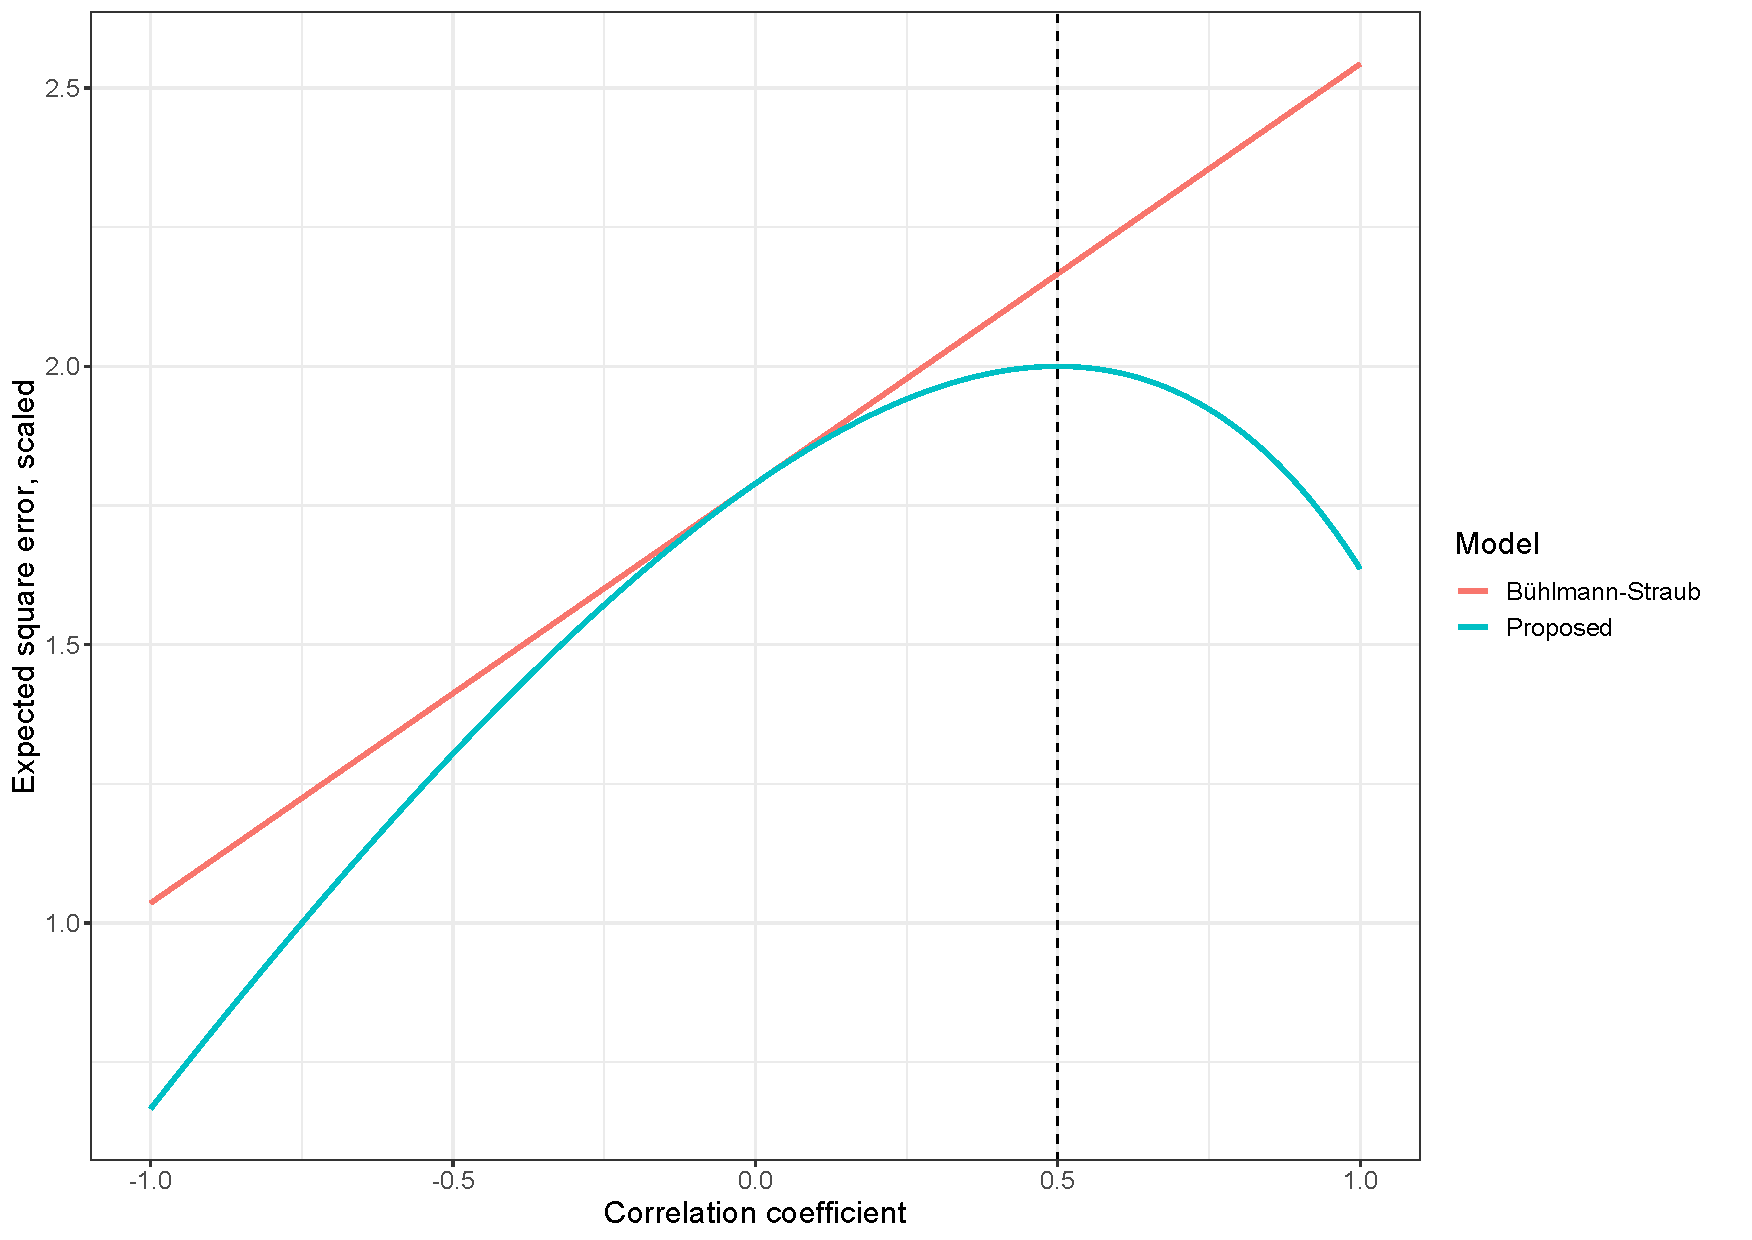
\includegraphics[width=0.75\textwidth]{2d_s.pdf}}
  \caption{Scaled expected square error of $\hat\mu$, see \eqref{eq:2d_error_s}, as a function of $\rho$ for the two models. A vertical line is drawn at $\rho=\rho^\ast$.}
  \label{fig:2d_s}
\end{figure}

\begin{figure}[H]
 \center
 \makebox[\textwidth][c]{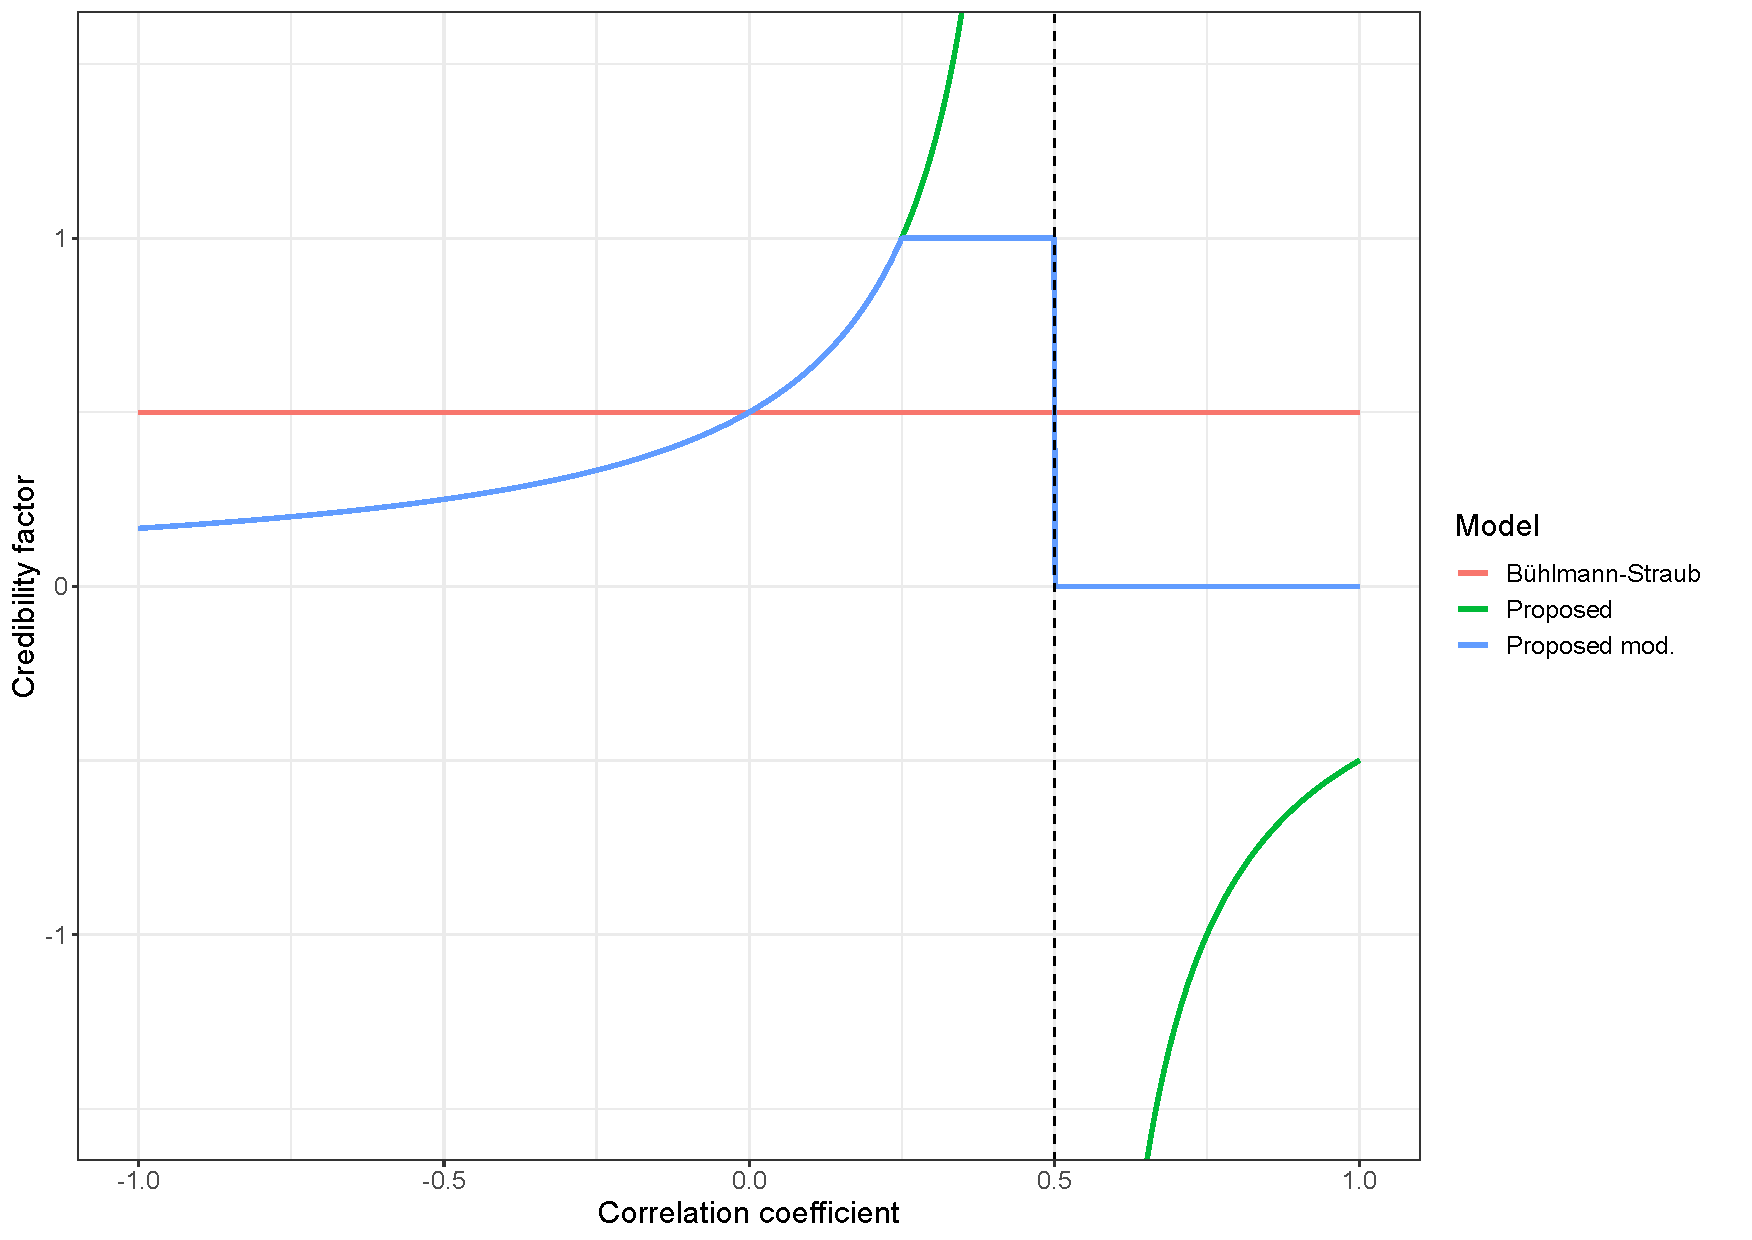
\includegraphics[width=0.75\textwidth]{2d_cred.pdf}}
  \caption{A comparison of the three candidates for the credibility factor. A vertical line is drawn at $\rho=\rho^\ast$.}
  \label{fig:2d_cred}
\end{figure}

\begin{figure}[H]
 \center
 \makebox[\textwidth][c]{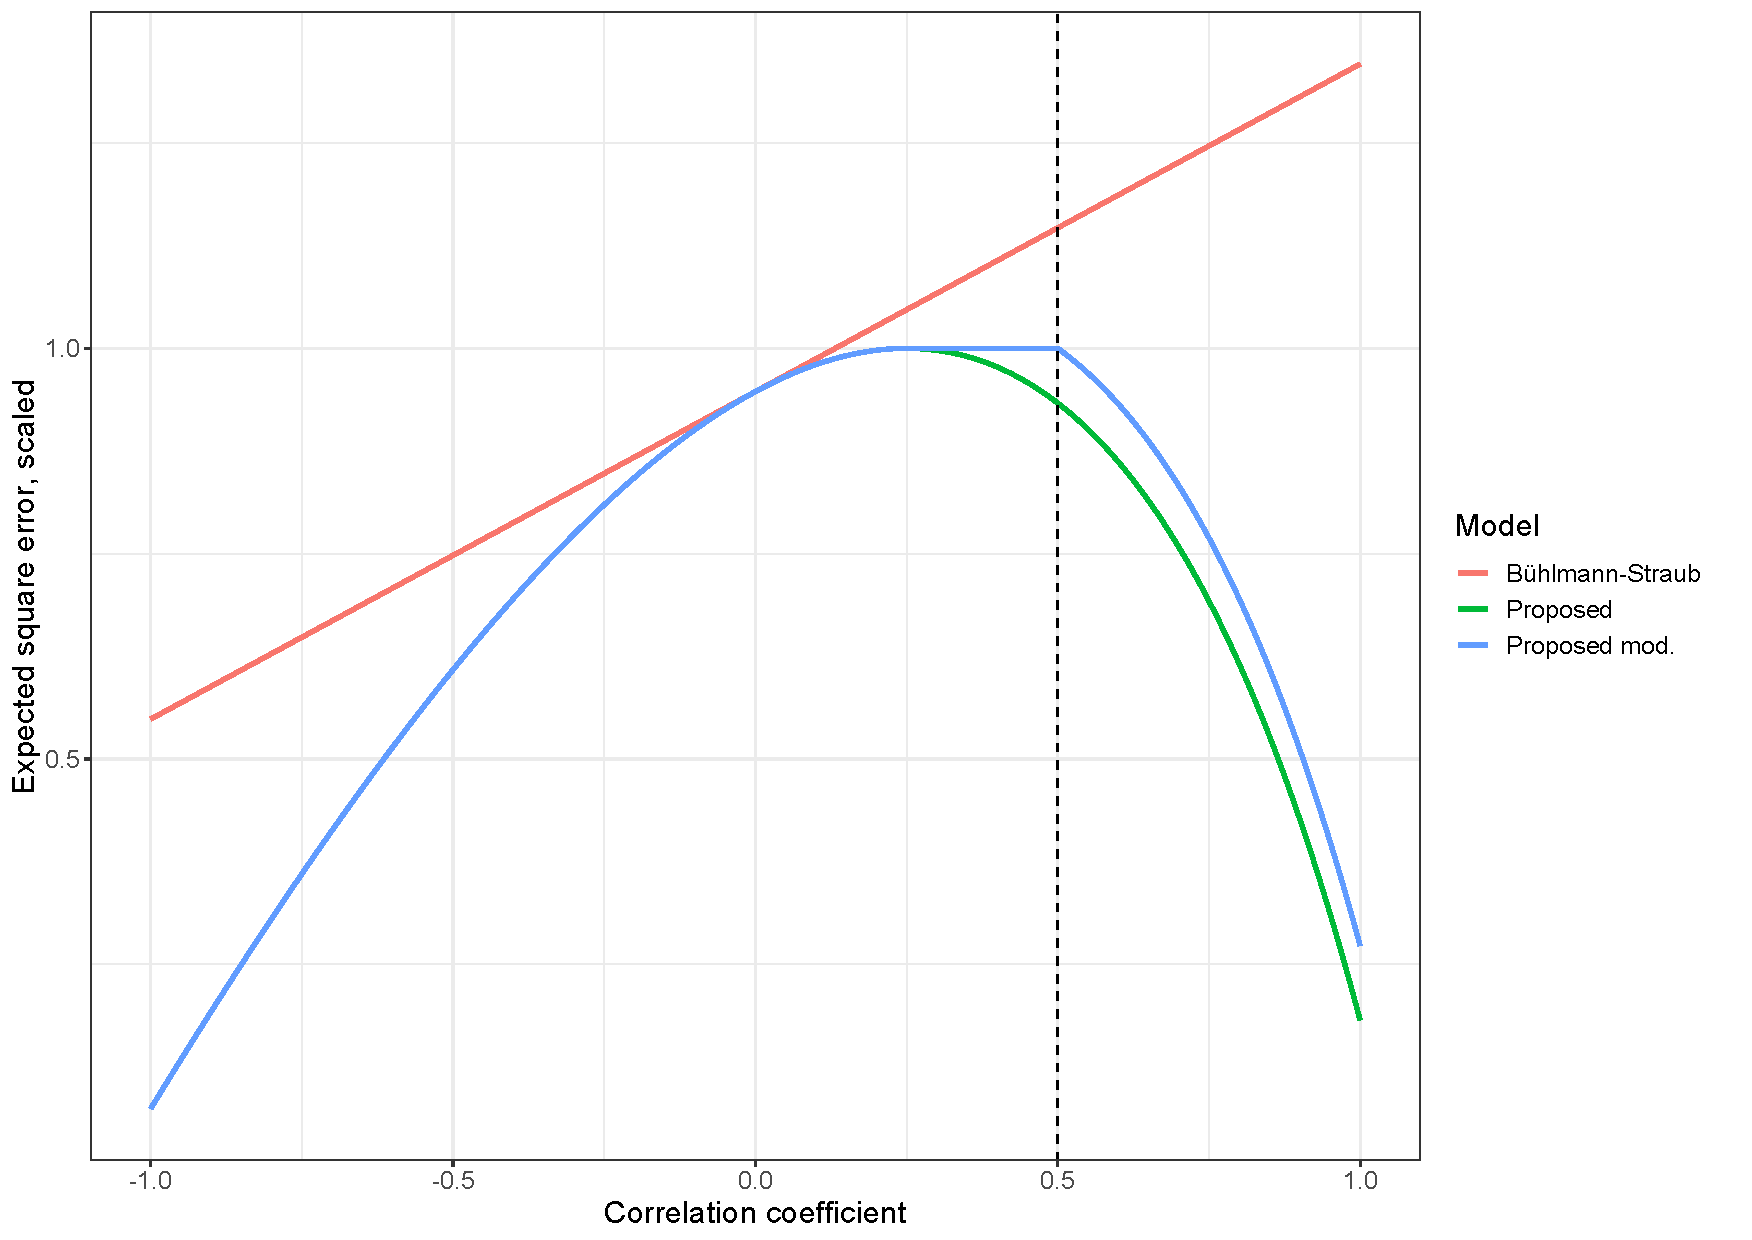
\includegraphics[width=0.75\textwidth]{2d_muj.pdf}}
  \caption{Scaled expected square error of $\hat\mu_j$, see \eqref{eq:2d_h_sigma}, as a function of $\rho$ for the three models. A vertical line is drawn at $\rho=\rho^\ast$.}
  \label{fig:2d_muj}
\end{figure}




\subsection{Parameter estimation}
In this section, we will construct unbiased estimators of the model parameters. We will do this for the special case when
\begin{equation*}
    \sigma_{jt}^2 = \frac{\sigma_j^2}{w_{jt}}.
\end{equation*}
The special case is similar to the Bühlmann-Straub model but with the extension that the base variance depends on the cohort. It is also an extension due to that $\rho_{ij}\neq\delta_{ij}$ in general.

By slightly modifying \eqref{eq:special_case_ajt} we see that the more general special case still implies \newline $a_{jt}=w_{jt}/w_{j\ast}$. Since the weights $w_{jt}$ are known it follows that the weights $a_{jt}$ are also known. 

For the covariance matrix $ K$ we will need the product $\sigma_{ij}^2\rho_{ij}$ as seen in \eqref{eq:K_bar}. By using \eqref{eq:sigma_ij} we can see that 
\begin{equation*}
    \begin{aligned}
        \sigma_{ij}^2\rho_{ij} &= \sum_t a_{it}a_{jt}\sigma_{it}\sigma_{jt}\rho_{ij} \\
        &= \rho_{ij}\sum_t \frac{w_{it}}{w_{i\ast}}\frac{w_{jt}}{w_{j\ast}}\frac{\sigma_i}{\sqrt{w_{it}}}\frac{\sigma_j}{\sqrt{w_{jt}}} \\
        &= \frac{\sigma_i\sigma_j\rho_{ij}}{w_{i\ast}w_{j\ast}}\sum_{t}\sqrt{w_{it}w_{jt}}.
    \end{aligned}
\end{equation*}
Because the weights $w_{jt}$ are known, the above relation tells us that if we can find an unbiased estimator for the product $\sigma_i\sigma_j\rho_{ij}$ then we also have an unbiased estimator for $\sigma_{ij}^2\rho_{ij}$. We may therefore write
\begin{equation}\label{eq:param_est_1}
    \reallywidehat{\sigma_{ij}^2\rho_{ij}} = \frac{\sum_t\sqrt{w_{it}w_{jt}}}{w_{i\ast}w_{j\ast}}\,\reallywidehat{\sigma_i\sigma_j\rho_{ij}}.
\end{equation}

Note that we only need to construct the unbiased estimators $\reallywidehat{\sigma_{ij}^2\rho_{ij}}$ and $\reallywidehat{\tau^2}$. This can be seen by inspecting \eqref{eq:proposed} and noting that $\sigma_{jj}^2$ can be written as $\sigma_{jj}^2\rho_{jj}$. I.e.\ we do not need to estimate $\sigma_{jj}^2$ separately.

We will start by searching for the unbiased estimator $\reallywidehat{\sigma_{ij}^2\rho_{ij}}$. Note first that
\begin{equation*}
\begin{aligned}
        \mathds{E}[(\mu_{it}-\hat\mu_i)(\mu_{jt}-\hat\mu_j)] &= \text{cov}(\mu_{it}-\hat\mu_i,\,\mu_{jt}-\hat\mu_j)+\mathds{E}[\mu_{it}-\hat\mu_i]\mathds{E}[\mu_{jt}-\hat\mu_j] \\
        &= \underbrace{\text{cov}(\mu_{it},\, \mu_{jt})}_{\circled{1}}-\underbrace{\text{cov}(\mu_{it},\, \hat\mu_j)}_{\circled{2}}-\underbrace{\text{cov}(\mu_{jt},\, \hat\mu_i)}_{\circled{3}}+\underbrace{\text{cov}(\hat\mu_i,\, \hat\mu_j)}_{\circled{4}}.
\end{aligned}
\end{equation*}
The expectations are zero since $\mathds{E}[\mu_{jt}]=\mathds{E}[\hat\mu_j]=\mu$ we only need to expand the covariance expression. The four terms can be expanded as follows
\begin{equation*}
    \begin{aligned}
        \circled{1}&= \bar K_{ij}^{tt} = \sigma_{it}\sigma_{jt}\rho_{ij}+\tau^2\delta_{ij}\\
        \circled{2}&=\sum_s a_{js}\text{cov}(\mu_{it},\, \mu_{js}) = \sum_s a_{js}\bar K_{ij}^{ts} = \sum_s a_{js}(\sigma_{it}\sigma_{js}\rho_{ij}\delta_{ts}+\tau^2\delta_{ij}) \\
        &= a_{jt}\sigma_{it}\sigma_{jt}\rho_{ij}+\tau^2\delta_{ij}\\
        \circled{3}&= a_{it}\sigma_{it}\sigma_{jt}\rho_{ij}+\tau^2\delta_{ij}\quad\quad\lbrace\text{by $j\rightarrow i$ in \circled{2}}\rbrace\\
        \circled{4}&=  K_{ij} = \sigma_{ij}^2\rho_{ij}+\tau^2\delta_{ij}.
    \end{aligned}
\end{equation*}
The $\tau^2\delta_{ij}$ terms cancel and we get
\begin{equation*}
\begin{aligned}
    \mathds{E}[(\mu_{it}-\hat\mu_i)(\mu_{jt}-\hat\mu_j)] &= \sigma_{it}\sigma_{jt}\rho_{ij} - a_{jt}\sigma_{it}\sigma_{jt}\rho_{ij} -a_{it}\sigma_{it}\sigma_{jt}\rho_{ij} + \sigma_{ij}^2\rho_{ij}\\
    &= (1-a_{it}-a_{jt})\sigma_{it}\sigma_{jt}\rho_{ij}+\sigma_{ij}^2\rho_{ij}\\
    &=\left(1-\frac{w_{it}}{w_{i\ast}}-\frac{w_{jt}}{w_{j\ast}}\right)\frac{\sigma_i\sigma_j\rho_{ij}}{\sqrt{w_{it}w_{jt}}}+\frac{\sigma_i\sigma_j\rho_{ij}}{w_{i\ast}w_{j\ast}}\sum_s\sqrt{w_{is}w_{js}}\\
    &= \left( \frac{w_{i\ast}w_{j\ast}-w_{it}w_{j\ast}-w_{jt}w_{i\ast}}{\sqrt{w_{it}w_{jt}}} + \sum_s \sqrt{w_{is}w_{js}}\right)\frac{\sigma_i\sigma_j\rho_{ij}}{w_{i\ast}w_{j\ast}}.
\end{aligned}
\end{equation*}
It follows that
\begin{equation*}
\begin{aligned}
&w_{i\ast}w_{j\ast}\mathds{E}\left[\sum_t \sqrt{w_{it}w_{jt}}(\mu_{it}-\hat\mu_i)(\mu_{jt}-\hat\mu_j)\right] \\
&=
    \left(\sum_t (w_{i\ast}w_{j\ast}-w_{it}w_{j\ast}-w_{jt}w_{i\ast}) + \sum_t \sqrt{w_{it}w_{jt}}\sum_s \sqrt{w_{is}w_{js}}\right)\sigma_i\sigma_j\rho_{ij}\\
&=  \left(Tw_{i\ast}w_{j\ast}-2w_{i\ast}w_{j\ast} + \left(\sum_t \sqrt{w_{it}w_{jt}}\right)^2\right)\sigma_i\sigma_j\rho_{ij}.
\end{aligned}
\end{equation*}
Thus the following estimator is unbiased
\begin{equation*}
    \reallywidehat{\sigma_i\sigma_j\rho_{ij}} = \frac{w_{i\ast}w_{j\ast}\sum_t \sqrt{w_{it}w_{jt}}(\mu_{it}-\hat\mu_i)(\mu_{jt}-\hat\mu_j)}{(T-2)w_{i\ast}w_{j\ast}+\left(\sum_t \sqrt{w_{it}w_{jt}}\right)^2}.
\end{equation*}
\eqref{eq:param_est_1} then yields
\begin{equation*}
    \reallywidehat{\sigma_{ij}^2\rho_{ij}} = \frac{\sum_t \sqrt{w_{it}w_{jt}}(\mu_{it}-\hat\mu_i)(\mu_{jt}-\hat\mu_j)}{\sum_t \sqrt{w_{it}w_{jt}}+(T-2)w_{i\ast}w_{j\ast}/\sum_t \sqrt{w_{it}w_{jt}}}.
\end{equation*}
What remains is to construct the unbiased estimator $\reallywidehat{\tau^2}$. First, observe that
\begin{equation*}
    \begin{aligned}
        \mathds{E}\left[\left(\hat\mu_j - \sum_i \frac{w_{i\ast}}{w_{\ast\ast}}\hat\mu_i\right)^2\right] &= \text{Var}\left(\hat\mu_j - \sum_i \frac{w_{i\ast}}{w_{\ast\ast}}\hat\mu_i\right) + \mathds{E}\left[\hat\mu_j - \sum_i \frac{w_{i\ast}}{w_{\ast\ast}}\hat\mu_i\right]^2.
    \end{aligned}
\end{equation*}
The second term on the right-hand side is zero since $\mathds{E}[\hat\mu_j]=\mu$ independently on the index $j$. Therefore, consider the following expansion of the variance.
\begin{equation}\label{eq:par_est_2}
\begin{aligned}
    \text{Var}\left(\hat\mu_j - \sum_i \frac{w_{i\ast}}{w_{\ast\ast}}\hat\mu_i\right) &= \text{Var}\left(\sum_i\left(\delta_{ij}- \frac{w_{i\ast}}{w_{\ast\ast}}\right)\hat\mu_i\right)\\
    &= \sum_{ik}\left(\delta_{ij}- \frac{w_{i\ast}}{w_{\ast\ast}}\right)\left(\delta_{kj}- \frac{w_{k\ast}}{w_{\ast\ast}}\right) K_{ik} \\
    &= \sum_{ik}\left(\delta_{ij}- \frac{w_{i\ast}}{w_{\ast\ast}}\right)\left(\delta_{kj}- \frac{w_{k\ast}}{w_{\ast\ast}}\right)\left(\sigma_{ik}^2\rho_{ik}+\tau^2\delta_{ik}\right).
\end{aligned}
\end{equation}
The expression above will be expanded in two steps. Consider first
\begin{equation*}
    \begin{aligned}
        &\sum_{ik}\left(\delta_{ij}- \frac{w_{i\ast}}{w_{\ast\ast}}\right)\left(\delta_{kj}- \frac{w_{k\ast}}{w_{\ast\ast}}\right)\sigma_{ik}^2\rho_{ik} \\
        &=\sum_{ik}\left( \delta_{ij}\delta_{kj} - \delta_{ij}\frac{w_{k\ast}}{w_{\ast\ast}}-\delta_{kj}\frac{w_{i\ast}}{w_{\ast\ast}}+\frac{w_{i\ast}w_{k\ast}}{w_{\ast\ast}^2}\right)\sigma_{ik}^2\rho_{ik} \\
        &= \sum_i \left( \delta_{ij}-2\frac{w_{i\ast}}{w_{\ast\ast}}\right)\sigma_{ij}^2\rho_{ij} + \sum_{ik}\frac{w_{i\ast}w_{k\ast}}{w_{\ast\ast}^2}\sigma_{ik}^2\rho_{ik}.
    \end{aligned}
\end{equation*}
Observe that the second term is a constant. Therefore it follows that
\begin{equation*}
\begin{aligned}
        &\sum_j \frac{w_{j\ast}}{w_{\ast\ast}} \sum_{ik}\left(\delta_{ij}- \frac{w_{i\ast}}{w_{\ast\ast}}\right)\left(\delta_{kj}- \frac{w_{k\ast}}{w_{\ast\ast}}\right)\sigma_{ik}^2\rho_{ik} \\
        &= \sum_{ij}\left( \frac{w_{j\ast}}{w_{\ast\ast}}\left( \delta_{ij}-2\frac{w_{i\ast}}{w_{\ast\ast}}\right)+\frac{w_{i\ast}w_{j\ast}}{w_{\ast\ast}^2}\right) \sigma_{ij}^2\rho_{ij} \\
        &= \sum_{j} \frac{w_{j\ast}}{w_{\ast\ast}} \underbrace{\sum_i \left(\delta_{ij}-\frac{w_{i\ast}}{w_{\ast\ast}}\right)\sigma_{ij}^2\rho_{ij}}_{\coloneqq c_j}.
\end{aligned}
\end{equation*}
Note that below is an unbiased estimator.
\begin{equation*}
    \hat c_j = \sum_i \left(\delta_{ij}-\frac{w_{i\ast}}{w_{\ast\ast}}\right)\reallywidehat{\sigma_{ij}^2\rho_{ij}}.
\end{equation*}
Now consider the weighted average of the second term in \eqref{eq:par_est_2}.
\begin{equation*}
    \begin{aligned}
        &\sum_j \frac{w_{j\ast}}{w_{\ast\ast}} \sum_{ik}\left(\delta_{ij}- \frac{w_{i\ast}}{w_{\ast\ast}}\right)\left(\delta_{kj}- \frac{w_{k\ast}}{w_{\ast\ast}}\right)\tau^2\delta_{ik} \\
        &= \sum_j \frac{w_{j\ast}}{w_{\ast\ast}} \sum_{i}\left(\delta_{ij}- \frac{w_{i\ast}}{w_{\ast\ast}}\right)^2\tau^2 \\
        &= \sum_j \frac{w_{j\ast}}{w_{\ast\ast}} \sum_{i}\left(\delta_{ij}^2+ \frac{w_{i\ast}^2}{w_{\ast\ast}^2} - 2\delta_{ij}\frac{w_{i\ast}}{w_{\ast\ast}}\right)\tau^2 \\
        &= \sum_j \frac{w_{j\ast}}{w_{\ast\ast}}\left(1+\sum_i \frac{w_{i\ast}^2}{w_{\ast\ast}^2} - 2\frac{w_{j\ast}}{w_{\ast\ast}}\right)\tau^2 \\
        &= \left(1 + \sum_i \frac{w_{i\ast}^2}{w_{\ast\ast}^2} - 2\sum_j \frac{w_{j\ast}^2}{w_{\ast\ast}^2}\right)\tau^2\\
        &= \left(1 -\sum_i \frac{w_{i\ast}^2}{w_{\ast\ast}^2}\right)\tau^2.
    \end{aligned}
\end{equation*}
We now have
\begin{equation*}
    \mathds{E}\left[\sum_j \frac{w_{j\ast}}{w_{\ast\ast}} \left(\hat\mu_j - \sum_i \frac{w_{i\ast}}{w_{\ast\ast}}\hat\mu_i\right)^2\right]=\sum_j \frac{w_{j\ast}}{w_{\ast\ast}}c_j + \left(1 -\sum_i \frac{w_{i\ast}^2}{w_{\ast\ast}^2}\right)\tau^2.
\end{equation*} 
From this, it follows that below is an unbiased estimator of $\tau^2$.
\begin{equation*}
\reallywidehat{\tau^2} = \frac{\sum_j \frac{w_{j\ast}}{w_{\ast\ast}}\left\{  \left(\hat\mu_j - \sum_i \frac{w_{i\ast}}{w_{\ast\ast}}\hat\mu_i\right)^2-\hat c_j \right\} }{1 -\sum_i w_{i\ast}^2/w_{\ast\ast}^2}.
\end{equation*}
The results of this section can be summarized as follows.
\begin{equation}\label{eq:param_est_final}
    \begin{dcases}
    \reallywidehat{\sigma_{ij}^2\rho_{ij}} &= \frac{\sum_t \sqrt{w_{it}w_{jt}}(\mu_{it}-\hat\mu_i)(\mu_{jt}-\hat\mu_j)}{\sum_t \sqrt{w_{it}w_{jt}}+(T-2)w_{i\ast}w_{j\ast}/\sum_t \sqrt{w_{it}w_{jt}}} \\
    \hat c_j &= \sum_i \left(\delta_{ij}-\frac{w_{i\ast}}{w_{\ast\ast}}\right)\reallywidehat{\sigma_{ij}^2\rho_{ij}} \\
\reallywidehat{\tau^2} &= \frac{\sum_j w_{j\ast}\left\{  \left(\hat\mu_j - \sum_i \frac{w_{i\ast}}{w_{\ast\ast}}\hat\mu_i\right)^2-\hat c_j \right\} }{w_{\ast\ast} -\sum_i w_{i\ast}^2/w_{\ast\ast}} \\
\hat{{K}}_{ij} &= \reallywidehat{\sigma_{ij}^2\rho_{ij}} + \reallywidehat{\tau^2}\delta_{ij}.
    \end{dcases}
\end{equation}
As a final note, due to its construction, $\reallywidehat{\tau^2}$ may come out negative. This is also a possibility in both the Bühlmann-Straub and Parodi-Bonche models. As suggested in \cite{buhlmann} (page 95 and consequently also in \cite{parodi} page 25) one may want to consider the following transformation instead
\begin{equation}\label{eq:tau_trans}
    \reallywidehat{\tau^2}^{+}=\max\left(\reallywidehat{\tau^2},\, 0\right).
\end{equation}
The transformed estimator will unfortunately be biased. Additionally, $\tau^2=0$ implies that there is no difference between the individual cohorts and we should therefore not consider them separately. This is in line with the fact that 
\begin{equation*}
    \lim_{\tau^2\to 0}z_{j}=0,
\end{equation*}
in the Bühlmann-Straub model and the proposed model.

Notice that the estimators for $\sigma_j$ are consistent between the two models. This can be seen by realizing that
\begin{equation}\label{eq:sigma_estimators_consistent}
    \reallywidehat{\frac{\sigma_j^2}{w_{j\ast}}} = \reallywidehat{\sigma_{jj}^2} =     
    \reallywidehat{\sigma_{jj}^2\rho_{jj}} = \frac{\sum_t w_{jt}(\mu_{jt}-\hat\mu_j)^2}{w_{j\ast}+(T-2)w_{j\ast}}=\frac{\hat\sigma_j^2}{w_{j\ast}},
\end{equation}
where $\hat\sigma_j$ is the Bühlmann-Straub estimator in \eqref{eq:buhlmann_estimators}.

\subsection{The balance property}
A set of credibility blended estimates $\hat\mu_j^b$ is said to satisfy the balance property if the following condition is met.
\begin{equation*}
    \sum_{jt} w_{jt}\mu_{jt} = \sum_{jt} w_{jt}\hat\mu_j^b.
\end{equation*}
Observe that the property is satisfied in expectation for any unbiased model. This follows from $\mathds{E}[\mu_{jt}]=\mathds{E}[\hat\mu_j^b]=\mu$.

Note that $w_{jt}\mu_{jt}$ is not a key ratio. Instead, it is the measurement $x_{jt}$ in the numerator of the key ratio. The balance property then states that the blended estimate is unbiased with respect to $x_{\ast\ast}$, i.e.\ the aggregation of measurements for the portfolio historically. As an example, suppose $x_{jt}$ is the aggregate loss amount for cohort $j$ over the term $t$. The blended estimate $\hat\mu_j^b$ then corresponds to a risk premium. The balance property states that if the insurer would have charged the risk premium historically, the net result would have been exactly 0.

We will now study the balance property closer for all models with $a_{jt}=w_{jt}/w_{j\ast}$. Consequently
\begin{equation*}
    \sum_t w_{jt}\mu_{jt} = w_{j\ast}\hat\mu_j.
\end{equation*}
Additionally, since $\hat\mu_j^b$ is independent on $t$ the balance property can be written as
\begin{equation*}
    \sum_j w_{j\ast}(\hat\mu_j - \hat\mu_j^b) = 0,
\end{equation*}
or
\begin{equation*}
    \sum_j w_{j\ast}(1-z_j)(\hat\mu_j - \hat\mu) = 0.
\end{equation*}
This condition is not satisfied in general. It is however satisfied by the Bühlmann-Straub model regardless of whether the underlying assumptions of the model are satisfied or not. To see this, note first that for the Bühlmann-Straub model, we have
\begin{equation*}
    w_{j\ast}(1-z_j)=w_{j\ast}\left(1 - \frac{w_{j\ast}}{w_{j\ast}+\kappa} \right) = \frac{w_{j\ast}\kappa}{w_{j\ast}+\kappa} = \kappa z_j,
\end{equation*}
and therefore also
\begin{equation*}
    \begin{aligned}
         \sum_j w_{j\ast}(1-z_j)(\hat\mu_j - \hat\mu) &= \sum_j \kappa z_j (\hat\mu_j - \hat\mu) \\
         &= \kappa \sum_j z_j\hat\mu_j - \kappa z_\ast \hat\mu \\
         &= 0,
    \end{aligned}
\end{equation*}
since $\hat\mu = \sum_j z_j \hat\mu_j / z_\ast$. We have thus shown that the balance property is always satisfied for the Bühlmann-Straub model regardless of whether the assumptions in \eqref{eq:special_case_1} are met or not.

\newpage
\section{Simulation study}
\subsection{Motivation}\label{sec:sim_motiv}
In this section, we will generate random but realistic data to which the proposed and Bühlmann-Straub models will be applied. The benefit of using simulated data is that the accuracy of the models can be easier assessed using the (mean) relative error since we have access to the true model parameters.

The basic idea is to run a large number of $N$ simulations and investigate the distribution of the relative errors in estimating $\mu$, $\mu_j$, and $\tau^2$. Since the proposed model does not satisfy the balance property in general the relative error for the aggregated measurements will be considered as well.

The simulations will be run for the special case 
\begin{equation*}
    \begin{cases}
        \sigma_{jt}^2 &= \sigma_j^2/w_{jt} \\
        \rho_{ij}&=\rho + (1-\rho)\delta_{ij}.
    \end{cases}
\end{equation*}
The second assumption states that all pair-wise correlations are identical and equal to $\rho$. In other words, $\rho_{ij}$ is the elements of a so-called equicorrelation matrix \cite{Oneill}. In practice the correlations will most likely not be equal, however, using a single correlation parameter should be good enough to capture the average overall correlation. It will also enable us to easier study the error's dependency on the correlation.

The parameters $\mu$, $\tau$, $J$, and $T$ will be considered fixed and will therefore not change between the simulations. The entities $\mu_j$, $w_{jt}$, $\mu_{jt}$ and $\sigma_j$ will be randomly generated for each simulation. When it comes to $\rho$ it turns out we cannot select any $\rho\in[-1,\, 1]$. Since variance is non-negative a lower bound for $\rho$ can be constructed as follows.
\begin{equation*}
    \begin{aligned}
    \text{Var}\left(\sum_j \upvarepsilon_{jt}\right) &\geq 0,\\
    \sum_j \text{Var}(\upvarepsilon_{jt}) + \sum_{i\neq j}\text{cov}(\upvarepsilon_{it},\, \upvarepsilon_{jt}) &\geq 0, \\
    J + J(J-1)\rho &\geq 0, \\
    \rho \geq \frac{1}{1-J}.
    \end{aligned}
\end{equation*}
The same result is also mentioned in \cite{Oneill}. For simulation $n\in[1,\, N]$ we therefore set
\begin{equation}\label{eq:rho_sim}
    \rho_n = \frac{N-1-J(n-1)}{(1-J)(N-1)}.
\end{equation}
For later reference, we will also define the following relative errors
\begin{align}
    \text{RE}_\mu &= (\hat\mu - \mu)/\mu \label{eq:RE_mu} \\
    \text{RE}_{\mu_j} &= \sum_j (\hat\mu_j^b - \mu_j)/\mu_j/J \label{eq:RE_muj} \\
    \text{RE}_\tau &= (\hat\tau^2 - \tau^2)/\tau^2 \label{eq:RE_tau}\\
    \text{RE}_\text{BP} &= \left.\left(\sum_j w_{j\ast}(\hat\mu_j^b -  \hat\mu_j)\right)\right/ \sum_j w_{j\ast}\hat\mu_j \label{eq:RE_bp}.
\end{align}
As a final note, we will use the "raw" estimators i.e.\ we will not use the transformations mentioned in \eqref{eq:tau_trans} or in \eqref{eq:2d_z_mod}.

\subsection{Parameter choice}
The following parameter choice is based on actuarial expert judgment and is considered realistic for transformed loss ratio data. Each cohort is thus a sub-portfolio within a larger portfolio. The key ratio corresponds to a loss ratio and the weights correspond to earned premium. This description is intentionally vague in order to protect company information. The actual choice is summarized in Table \ref{tab:parameters}. As can be seen, the parameter table states that we are studying 9 cohorts over 10 terms. 

With the current parameter choice, it is possible that $\mu_{jt}$ is negative. Although this seems strange for a loss ratio it is not a problem for the model itself.

\begin{table}[H]
\centering
\caption{Parameter choice for simulation study}
\label{tab:parameters}
\begin{tabular}{ccc}
\hline
Variable     & Sampled from, if random  & Value, if fixed \\ \hline
$\mu$ && 1 \\
$\tau$ && 0.6 \\
$J$ && 9 \\
$T$ && 10 \\
$N$ && $10^5$ \\
$\mu_j$ & $\Gamma (\mu^2/\tau^2,\, \mu/\tau^2)$ &\\
$\sigma_j^2$ &  $\text{Lognormal}(16,\, \sqrt{2})$ &\\
$w_j$ & $\mathcal{N}(3\cdot 10^7,\, 3\cdot 10^5)$ &\\
$w_{jt}$ & $\mathcal{N}(w_j,\, w_j/10)$& \\
\hline
\end{tabular}
\end{table}

\subsection{Simulation procedure}
In this subsection, we describe how the data, ultimately $\mu_{jt}$, is generated. We do this by defining a couple of simulation steps as follows.
\begin{enumerate}
    \item Set simulation fixed parameters according to Table \ref{tab:parameters} and simulation counter $n$ to $1$.
    \item Construct the $n$th equicorrelation matrix by using \eqref{eq:rho_sim}. 
    \item Generate the random parameters according to Table \ref{tab:parameters}.
    \item Generate the matrix elements $\upvarepsilon_{jt}$ with columns drawn from a multivariate normal distribution with zero mean vector and covariance matrix equal to the equicorrelation matrix.
    \item Generate the data points by the identity $\mu_{jt}=\mu_j + \sigma/\sqrt{w_{jt}} \cdot \upvarepsilon_{jt}$.
    \item Estimate model parameters and evaluate the model. Calculate the relative errors $\text{RE}_x$ defined in Section \ref{sec:sim_motiv}.
    \item Go back to step 2 and increment $n$ by 1. Stop once $n=N$ is reached.
\end{enumerate}
Once the data points have been generated (step 5) the proposed and Bühlmann-Straub models are evaluated using \eqref{eq:proposed} and \eqref{eq:buhlmann} respectively. The model parameters are estimated using \eqref{eq:param_est_final} and \eqref{eq:buhlmann_estimators} respectively.

\subsection{A single simulation}
For illustrative purposes, one out of the $N$ simulations will be investigated in closer detail. Specifically, we will use the first simulation, meaning that $\rho = \rho_1 = -0.125$. Remember that we are studying 9 cohorts over 10 insurance periods.

In Table \ref{tab:1_sim_w} and in Table \ref{tab:1_sim_mu} the weights and key ratios can be seen respectively. In Table \ref{tab:1_sim_eval} the two models have been evaluated. A part of the table has been visualized in Figure \ref{fig:1_sim} as well. 

Due to \eqref{eq:special_case_ajt} and \eqref{eq:sigma_estimators_consistent} the estimators $\hat\mu_j$ and $\hat\sigma_{jj}$ are identical between the two models. The models are only different in $\hat\mu$, $z_j$, and $\hat\mu_j^b$. This explains the structure of Table \ref{tab:1_sim_eval}.

The proposed model contains an estimator for the correlation matrix. The outcome of the estimator can be seen in Table \ref{tab:1_sim_corr}. Notice that the estimator in \eqref{eq:param_est_final} could be improved if the correlation was assumed to be identical between the cohorts. Since this is not the case here the proposed model will in a sense overfit the correlations. The average of the elements in the lower diagonal of the correlation matrix can be seen in Table \ref{tab:1_sim_single_params} and we see that it is fairly close to the actual value nevertheless. Remember that the Bühlmann-Straub model has no estimator for the correlation.

The relative errors as defined in Section \ref{sec:sim_motiv} are shown in Table \ref{tab:1_sim_errors}. For the first simulation, the proposed model estimated $\tau$ noticeably better than the Bühlmann-Straub model. It also performed somewhat better at estimating the vector of elements $\mu_j$ when using the blended estimate, although both models performed quite badly in this simulation. No noticeable difference can be seen when estimating $\hat\mu$. Finally, a slight error in the balance property is seen for the proposed model as expected.

\begin{table}[H]
\label{tab:1_sim_w}
\centering
\caption{Weights $w_{jt}$ in millions for the first simulation}
\begin{tabular}{rrrrrrrrrrr}
  \hline
 $j\,\backslash\, t$& 1 & 2 & 3 & 4 & 5 & 6 & 7 & 8 & 9 & 10 \\ 
  \hline
1 & 2.9 & 2.5 & 2.1 & 2.3 & 2.3 & 2.5 & 2.5 & 2.6 & 2.5 & 2.6 \\ 
  2 & 3.7 & 3.5 & 3.1 & 3.1 & 2.7 & 3.2 & 3.4 & 2.7 & 3.1 & 3.8 \\ 
  3 & 3.7 & 2.8 & 3.1 & 3.1 & 3.2 & 2.4 & 2.7 & 2.9 & 3.1 & 2.6 \\ 
  4 & 2.9 & 3.0 & 2.9 & 1.9 & 3.0 & 3.2 & 2.8 & 2.2 & 2.9 & 2.6 \\ 
  5 & 3.5 & 3.5 & 3.2 & 2.8 & 3.2 & 3.3 & 3.6 & 3.1 & 3.0 & 3.7 \\ 
  6 & 3.0 & 2.9 & 3.0 & 2.9 & 2.5 & 2.5 & 2.8 & 3.4 & 2.4 & 2.9 \\ 
  7 & 3.2 & 3.5 & 2.9 & 3.5 & 3.1 & 3.8 & 3.3 & 3.4 & 3.2 & 3.1 \\ 
  8 & 2.4 & 2.1 & 2.6 & 2.9 & 2.7 & 2.8 & 2.8 & 2.9 & 2.1 & 2.4 \\ 
  9 & 3.5 & 2.7 & 3.4 & 3.1 & 3.1 & 3.2 & 3.1 & 3.6 & 3.1 & 3.2 \\ 
   \hline
\end{tabular}
\end{table}

\begin{table}[H]
\label{tab:1_sim_mu}
\centering
\caption{Data points $\mu_{jt}$ for the first simulation}
\begin{tabular}{rrrrrrrrrrr}
  \hline
 $j\,\backslash\, t$& 1 & 2 & 3 & 4 & 5 & 6 & 7 & 8 & 9 & 10 \\ 
  \hline
1 & 5.00 & -3.16 & -0.61 & -0.77 & 1.12 & 1.09 & -0.23 & 2.22 & -1.24 & 1.21 \\ 
  2 & 3.11 & 1.33 & 3.08 & 0.98 & -0.81 & 1.86 & -2.05 & 2.05 & 3.28 & 2.10 \\ 
  3 & -0.98 & -1.03 & -0.52 & -0.16 & 1.21 & 1.30 & 4.77 & -1.25 & 0.98 & 0.08 \\ 
  4 & 1.74 & 0.36 & 0.53 & 0.82 & 1.24 & -0.28 & 0.36 & 0.96 & 2.98 & 2.70 \\ 
  5 & -7.38 & -0.47 & 0.19 & 4.07 & 1.88 & 1.09 & -2.26 & 3.68 & 3.25 & 0.23 \\ 
  6 & -3.19 & 4.42 & 1.56 & 0.10 & -1.60 & -1.13 & -0.48 & -2.93 & -2.72 & -0.58 \\ 
  7 & 1.21 & 0.14 & 0.82 & 0.98 & 0.91 & 1.98 & 1.24 & 0.22 & -1.69 & 0.46 \\ 
  8 & 3.04 & 6.56 & 1.68 & 3.65 & 2.05 & 1.97 & 4.20 & 0.39 & 4.00 & -0.38 \\ 
  9 & 1.36 & 0.63 & 0.30 & -1.33 & 0.08 & -0.99 & 0.33 & 1.85 & -0.52 & -0.43 \\ 
   \hline
\end{tabular}
\end{table}

\begin{table}[H]
\label{tab:1_sim_eval}
\centering
\caption{Model evaluation for the proposed and Bühlmann-Straub models for the first simulation}
\begin{tabular}{rrrrrrrrrrrr}
  \hline
 $j$ & $w_{j\ast}\cdot 10^{-5}$ & $\sigma_{jj}$ & $\hat\sigma_{jj}$ & $\mu_j$ & $\hat\mu_j$ & $\hat\mu$ & $\hat\mu^B$ & $z_j$ & $z_j^B$ & $\hat\mu_j^b$ & $\hat\mu_j^{b,B}$ \\ 
  \hline
  1 & 2487 & 0.65 & 0.73 & 1.05 & 0.55 & 0.7173 & 0.7180 & 0.38 & 0.48 & 0.65 & 0.64 \\ 
  2 & 3244 & 0.64 & 0.55 & 0.83 & 1.52 & 0.7173 & 0.7180 & 0.53 & 0.54 & 1.14 & 1.15 \\ 
  3 & 2968 & 0.54 & 0.55 & 1.08 & 0.37 & 0.7173 & 0.7180 & 0.52 & 0.52 & 0.54 & 0.54 \\ 
  4 & 2738 & 0.33 & 0.34 & 0.98 & 1.12 & 0.7173 & 0.7180 & 0.74 & 0.50 & 1.02 & 0.92 \\ 
  5 & 3271 & 0.76 & 1.08 & 0.34 & 0.24 & 0.7173 & 0.7180 & 0.23 & 0.54 & 0.61 & 0.46 \\ 
  6 & 2837 & 0.65 & 0.74 & 0.97 & -0.65 & 0.7173 & 0.7180 & 0.38 & 0.51 & 0.19 & 0.02 \\ 
  7 & 3302 & 0.30 & 0.31 & 0.15 & 0.65 & 0.7173 & 0.7180 & 0.77 & 0.55 & 0.66 & 0.68 \\ 
  8 & 2565 & 0.73 & 0.61 & 1.70 & 2.63 & 0.7173 & 0.7180 & 0.48 & 0.48 & 1.63 & 1.64 \\ 
  9 & 3196 & 0.39 & 0.32 & 0.10 & 0.16 & 0.7173 & 0.7180 & 0.76 & 0.54 & 0.29 & 0.42 \\ 
   \hline
\end{tabular}
\end{table}

\begin{table}[H]
\label{tab:1_sim_corr}
\centering
\caption{Estimated correlation matrix for the proposed model for the first simulation}
\begin{tabular}{r|rrrrrrrrr}
  \hline
 $j\,\backslash\, j$ & 1 & 2 & 3 & 4 & 5 & 6 & 7 & 8 & 9 \\ 
  \hline
1 & 1.000 & 0.220 & -0.188 & 0.191 & -0.503 & -0.756 & 0.381 & -0.547 & 0.439 \\ 
  2 & 0.220 & 1.000 & -0.738 & 0.396 & -0.041 & -0.155 & -0.351 & -0.257 & 0.099 \\ 
  3 & -0.188 & -0.738 & 1.000 & -0.153 & -0.028 & -0.084 & 0.177 & 0.198 & -0.329 \\ 
  4 & 0.191 & 0.396 & -0.153 & 1.000 & 0.020 & -0.443 & -0.694 & -0.227 & -0.008 \\ 
  5 & -0.503 & -0.041 & -0.028 & 0.020 & 1.000 & 0.048 & -0.357 & -0.202 & -0.418 \\ 
  6 & -0.756 & -0.155 & -0.084 & -0.443 & 0.048 & 1.000 & 0.057 & 0.490 & -0.211 \\ 
  7 & 0.381 & -0.351 & 0.177 & -0.694 & -0.357 & 0.057 & 1.000 & -0.167 & -0.075 \\ 
  8 & -0.547 & -0.257 & 0.198 & -0.227 & -0.202 & 0.490 & -0.167 & 1.000 & -0.113 \\ 
  9 & 0.439 & 0.099 & -0.329 & -0.008 & -0.418 & -0.211 & -0.075 & -0.113 & 1.000 \\ 
   \hline
\end{tabular}
\end{table}

\begin{table}[H]
\label{tab:1_sim_single_params}
    \centering
        \caption{Estimation outcome for the model parameters for the first simulation}
    \begin{tabular}{rrrr}
    \hline
    Parameter & True value & Proposed estimator & Bühlmann-Straub estimator \\
    \hline
    $\mu$ & 1 & 0.7173 & 0.7180 \\
    $\tau$ & 0.6 & 0.617 & 0.652 \\
    $\rho$ & -0.125 & -0.120 & 0 \\    
    \hline
    \end{tabular}
\end{table}

\begin{table}[H]
\label{tab:1_sim_errors}
    \centering
        \caption{Summary of the relative errors in percent for the first simulation}
    \begin{tabular}{rrrr}
    \hline
    Error type & Proposed model & Bühlmann-Straub model \\
    \hline
    $\text{RE}_\tau$ & 5.66      & 18.02\\
    $\text{RE}_{\mu_j}$ & 54.79  & 62.47 \\
    $\text{RE}_\mu$ &  -28.27    & -28.20 \\
    $\text{RE}_\text{BP}$ & 4.07 & 0 \\  
    \hline
    \end{tabular}
\end{table}

\begin{figure}[H]
 \center
 \makebox[\textwidth][c]{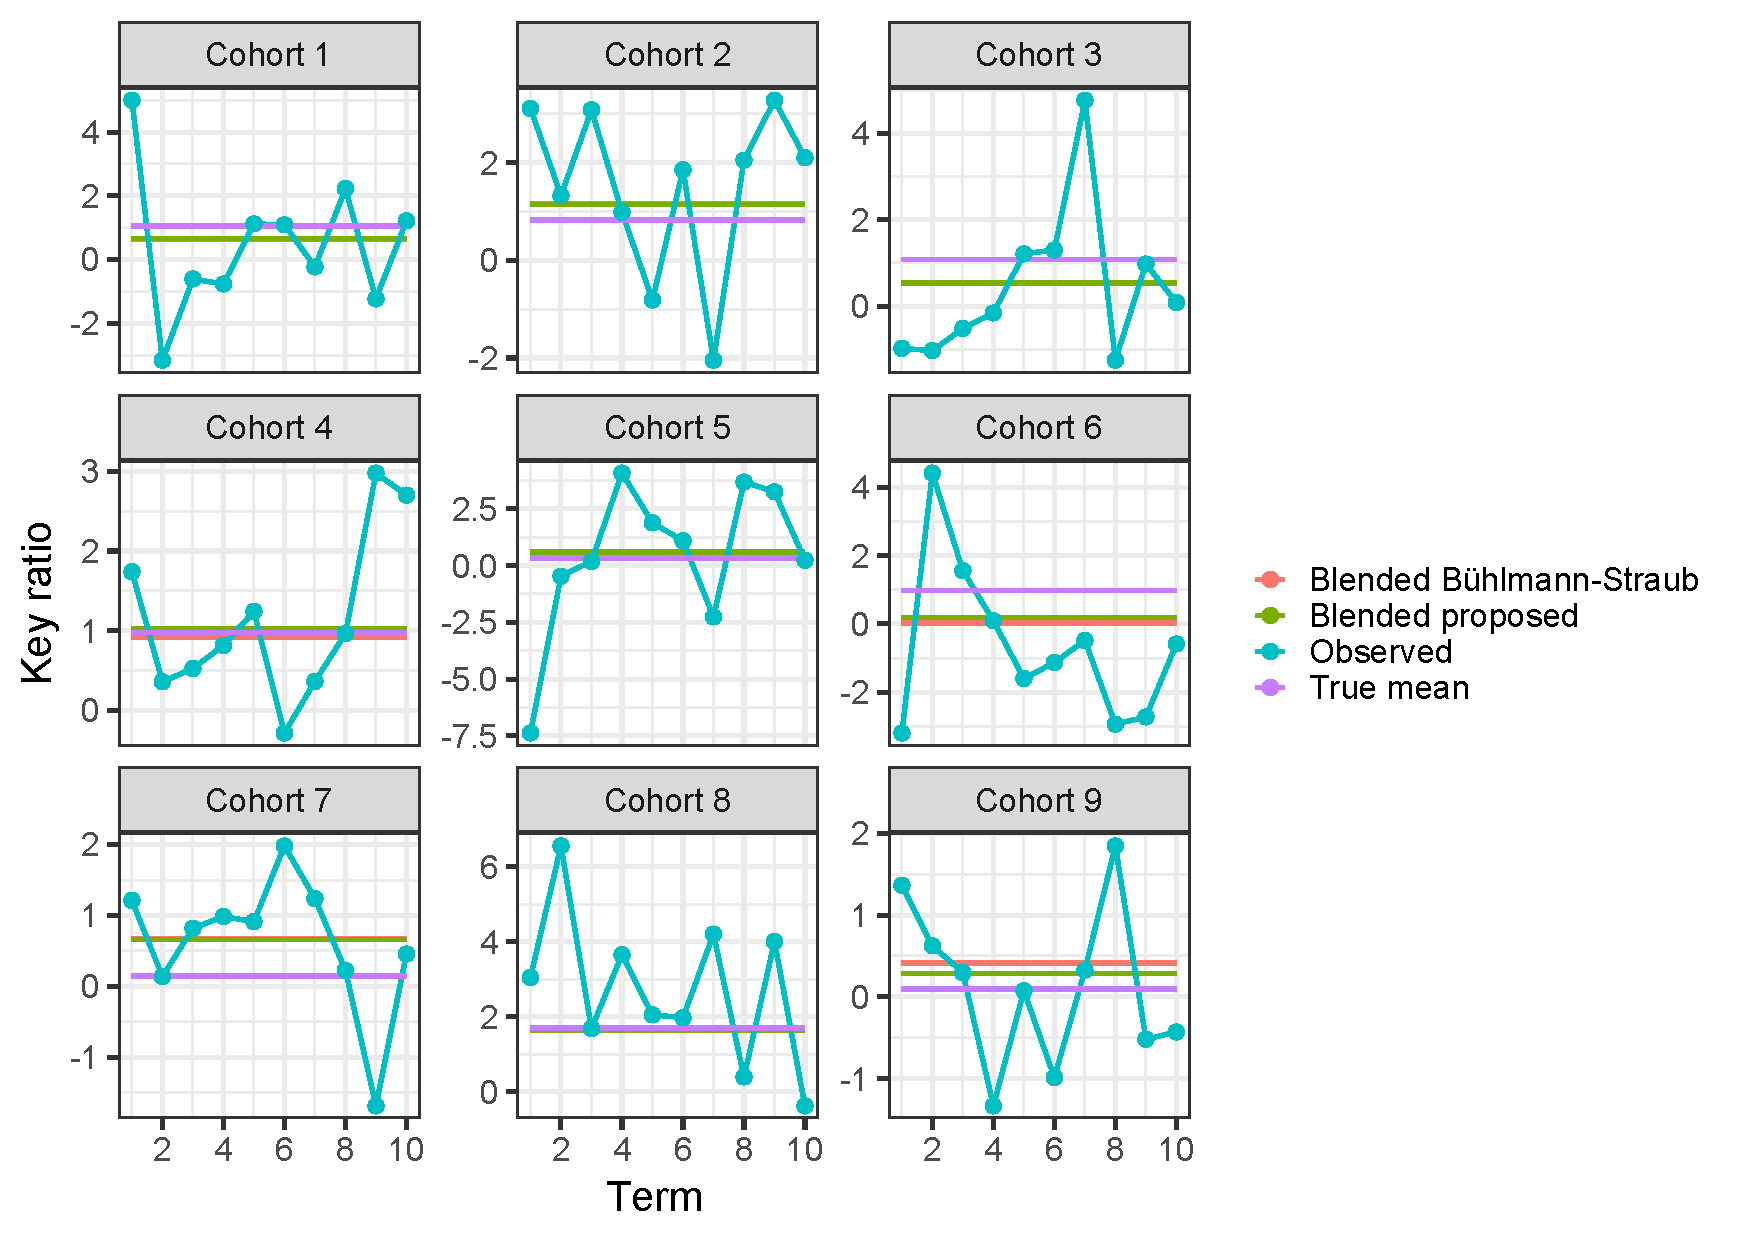
\includegraphics[width=.95\textwidth]{1_sim.pdf}}
  \caption{A visualization of the first simulation in the series of $N$ simulations.}
  \label{fig:1_sim}
\end{figure}

\subsection{All $N$ simulations}
Now we will perform a similar analysis as in the previous subsection but averaged over all $N$ runs. 

We will use a pseudo-log scale for the visualization of the relative error distributions. The pseudo-log transform is defined as
\begin{equation*}
    \texttt{psuedo\_log}\,(x) \coloneqq \text{arsinh}\left(\frac{x}{2}\right) = \text{ln}\left(\frac{x}{2}+ \sqrt{\left(\frac{x}{2}\right)^2+1}\right).
\end{equation*}
This transformation retains the sign of the original variable while at the same time behaving like the regular log transform for large $x$. Since the relative errors will span across multiple orders of magnitude a log-like transformation will help visualize the data. In Figure \ref{fig:trans} the transformation has been visualized and can be compared to the natural logarithm and identity transformations.

The large variance in the proposed model is mainly due to singularities in $z_j$ and $b_j$. Similar to what we saw in the two-dimensional special case previously. If the estimated parameters happen to be close to the points of singularity the error may be magnified quite significantly.

We will start by inspecting density plots for the relative errors. Please see Figures \ref{fig:err_dist_mu}, \ref{fig:err_dist_muj}, \ref{fig:err_dist_tau} and \ref{fig:err_dist_bp}. A summary is also available in Table \ref{tab:avg_errors}.

For all targets, except for $\tau$, and for both models, the median relative error is lower than the average relative error. This indicates that outlier behavior is driving the average relative error. This likely originates from the heavy tail in the random data connected to the log-normal distribution assigned to $\sigma_{j}^2$. If one focuses on the mode of the density plots it is more clear that the proposed model outperforms the Bühlmann-Straub model in the simulations.

The blended estimate from the proposed model seems to outperform the Bühlmann-Straub model at estimating $\mu_j$. This comes at the cost of losing the balance property, but only by a couple of percents in the median. 

The same data can also be plotted as a function of the correlation coefficient. Please see Figures \ref{fig:err_trend_mu}, \ref{fig:err_trend_muj}, \ref{fig:err_trend_tau} and \ref{fig:err_trend_bp}. Since we already have the overall average from the summary statistics it would be of added interest to consider local averages. The local average is studied using the function \texttt{ggplot2::geom\_smooth}() in \texttt{R}. By default, it uses a GAM with smoothing. The exact details of the trend line are not of interest here, as long as it is flexible enough. 

The accuracy of the proposed model seems to be independent of $\rho$. This is good because otherwise, it would indicate there is still some bias left in the estimators. It is interesting to see that both models seem to be performing equally well at estimating $\mu$ when less focus is put on extreme values. The benefit of the proposed model seems to be a growing function of $\rho$ when estimating $\mu_j$ and $\tau$. Most notably so for $\mu_j$.

\begin{figure}[H]
 \center
 \makebox[\textwidth][c]{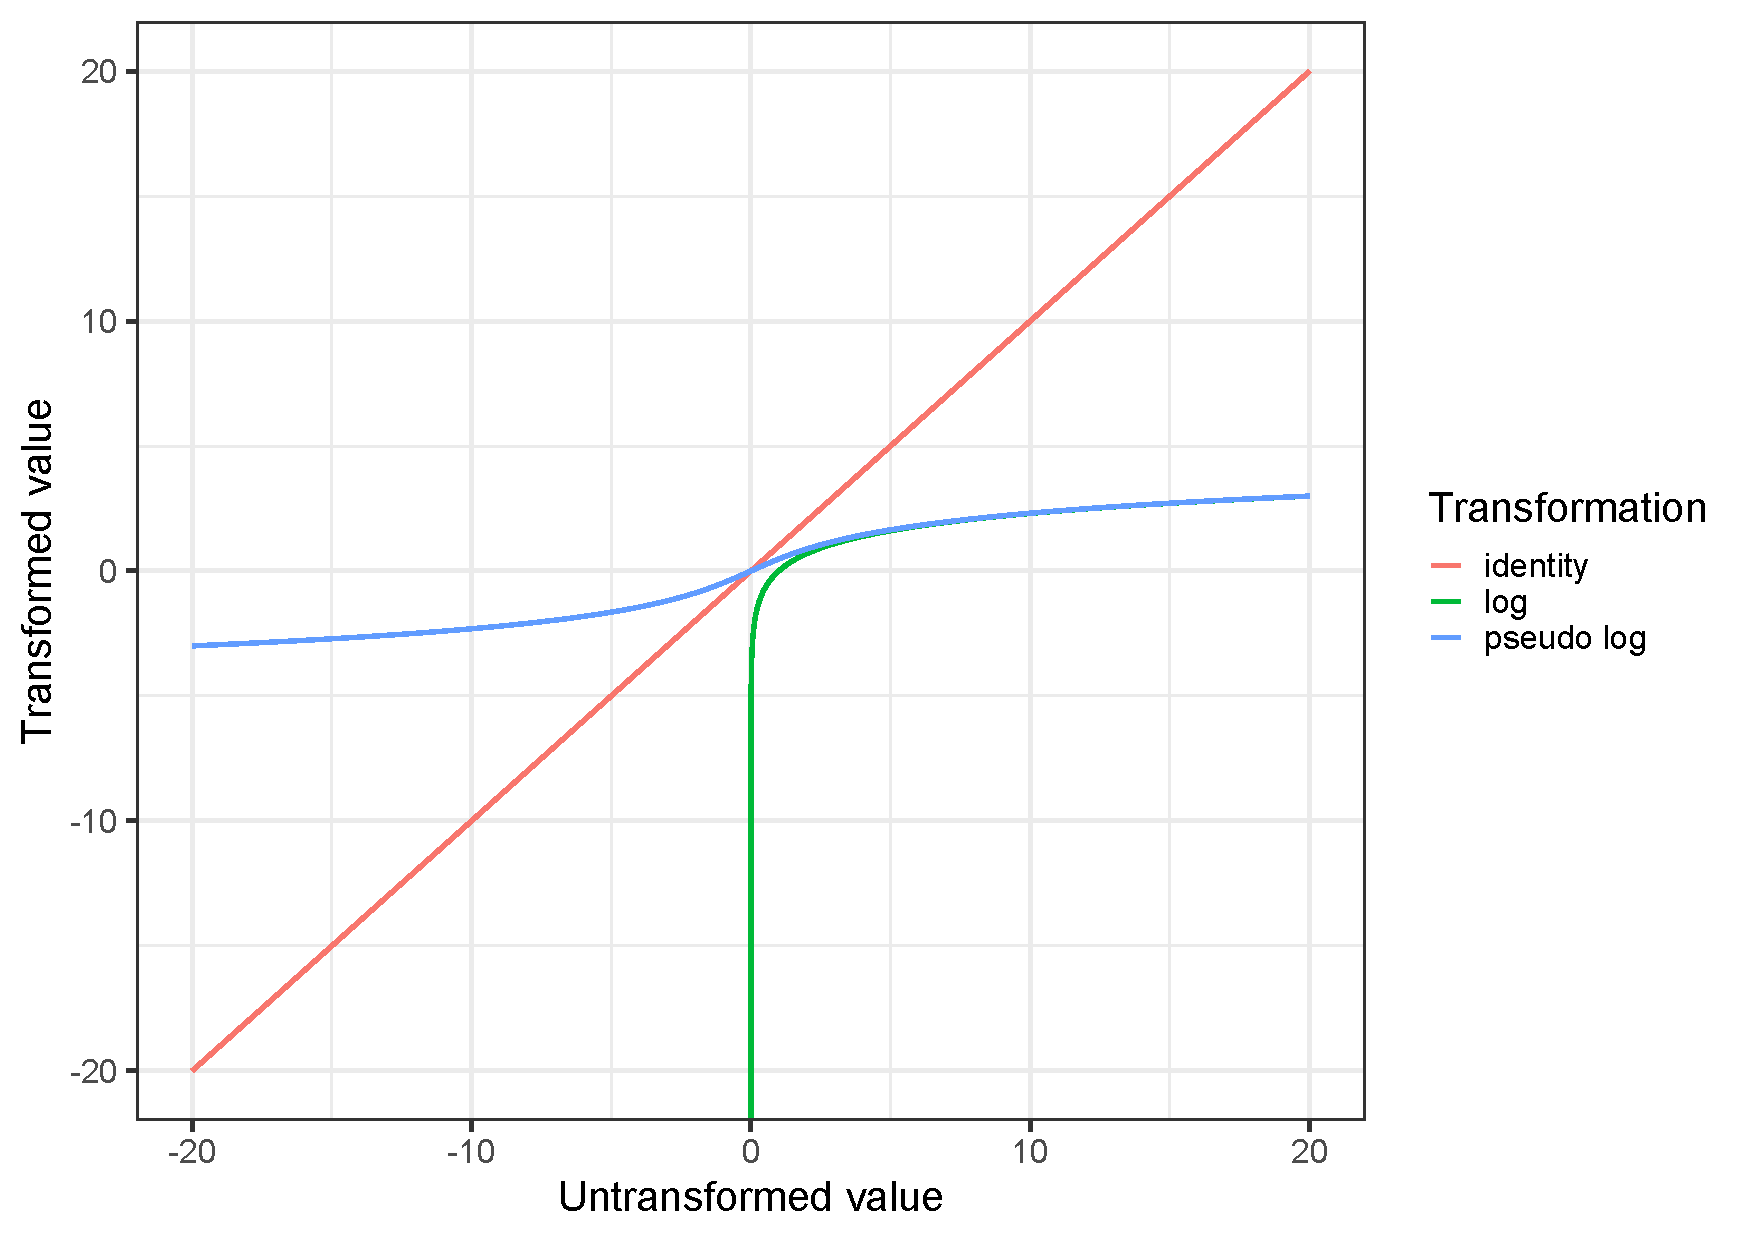
\includegraphics[width=.7\textwidth]{trans.pdf}}
  \caption{A comparison of the transformation candidates used for scaling the relative errors.}
  \label{fig:trans}
\end{figure}

\begin{table}[H]
\label{tab:avg_errors}
    \centering
        \caption{Summary statistics in percent for the relative errors for the two models over $10^5$ simulations.}
    \begin{tabular}{lcccc}
    \hline
    Error type & \multicolumn{2}{c}{Proposed model} & \multicolumn{2}{c}{Bühlmann-Straub model} \\
    & Average & Median &  Average & Median\\
    \hline
    $\text{RE}_\mu$ & -10.4 & 0.5 & 0.4 & -0.1 \\
    $\text{RE}_{\mu_j}$ & -22.3 & 16.7 & 55.0 & 39.4 \\
    $\text{RE}_\tau$  & -0.9 & -33.7 & -60.2 & -77.6 \\
    $\text{RE}_\text{BP}$ & -15.1 & -2.7 & 0 & 0 \\
    \hline
    \end{tabular}
\end{table}

\begin{figure}[H]
 \center
 \makebox[\textwidth][c]{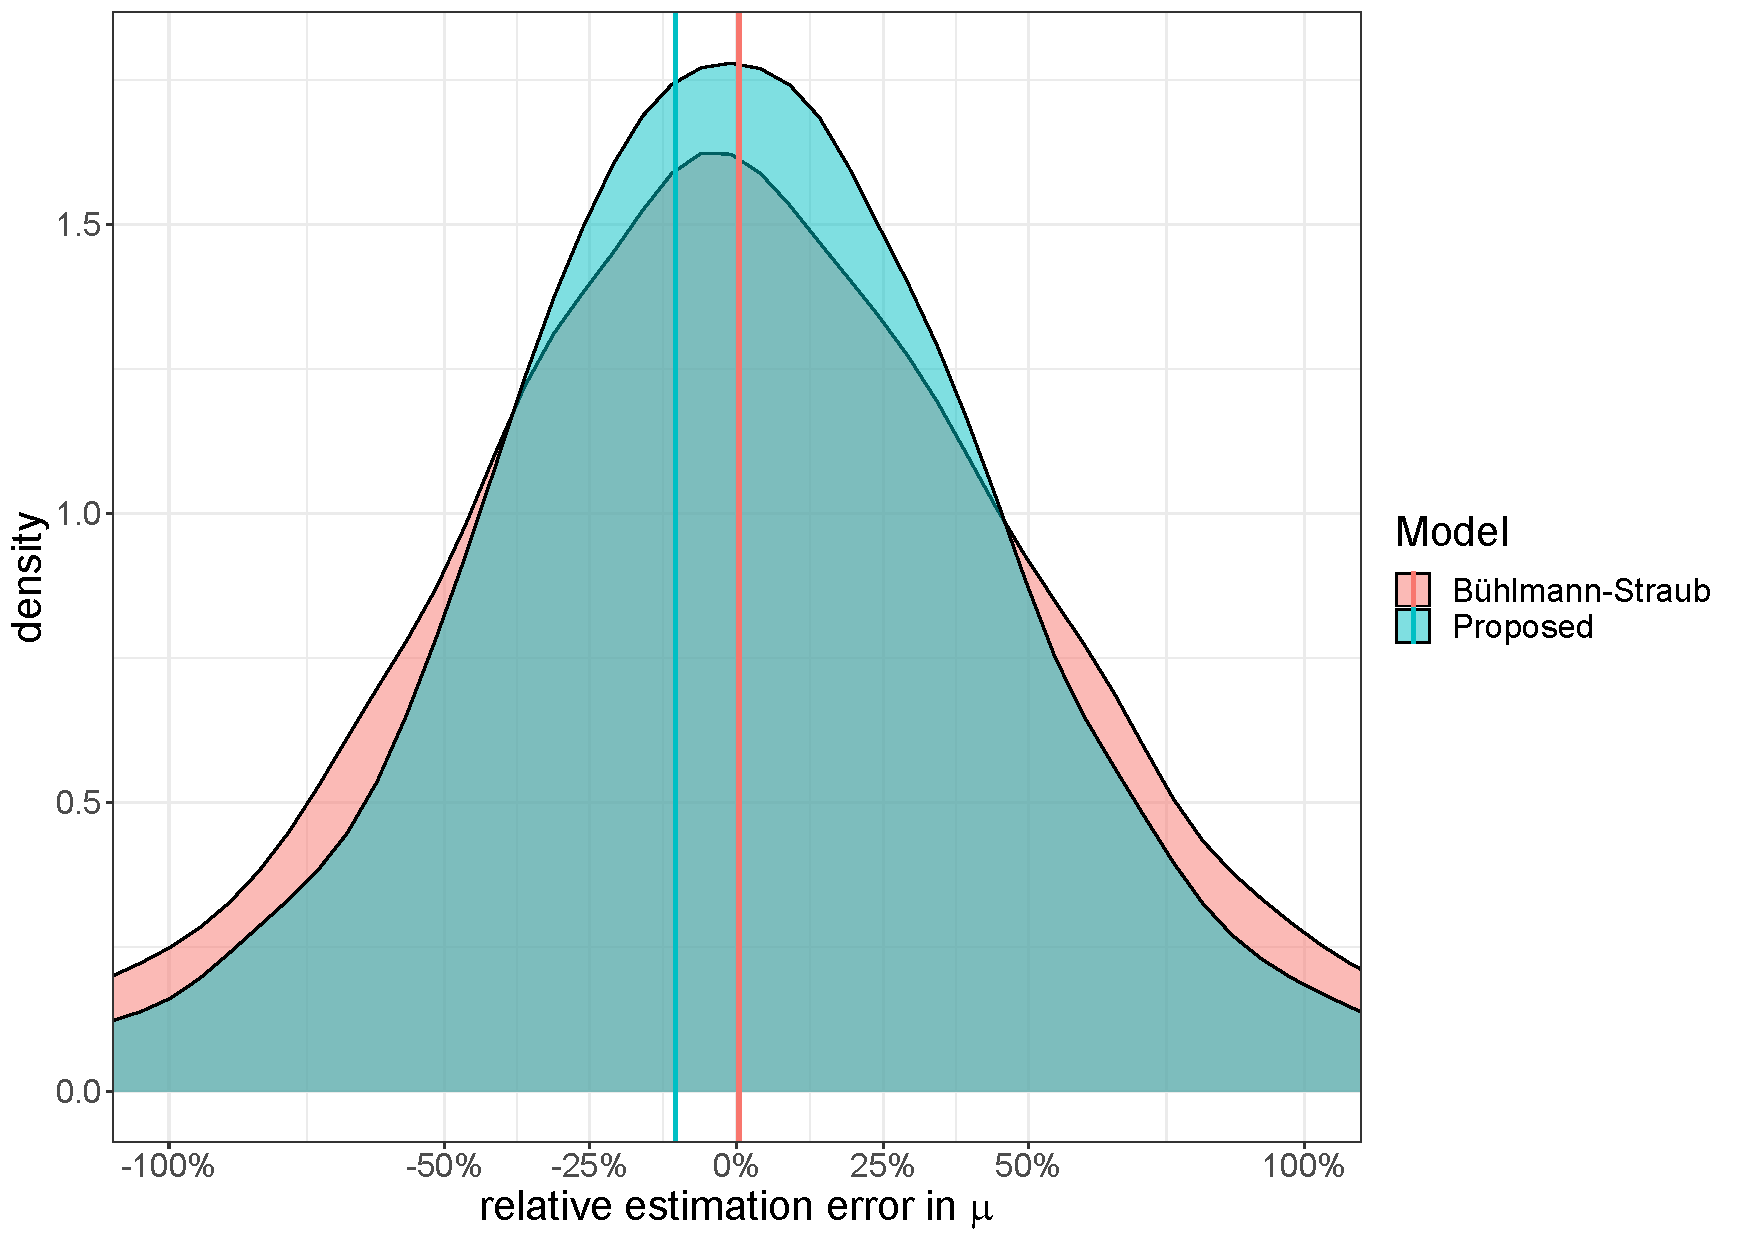
\includegraphics[width=.74\textwidth]{err_dist_mu.pdf}}
  \caption{The distribution of relative error in the estimator $\hat\mu$ as defined in \eqref{eq:RE_mu} over $10^5$ simulations for the two models. A vertical line is drawn at the average.}
  \label{fig:err_dist_mu}
\end{figure}
\begin{figure}[H]
 \center
 \makebox[\textwidth][c]{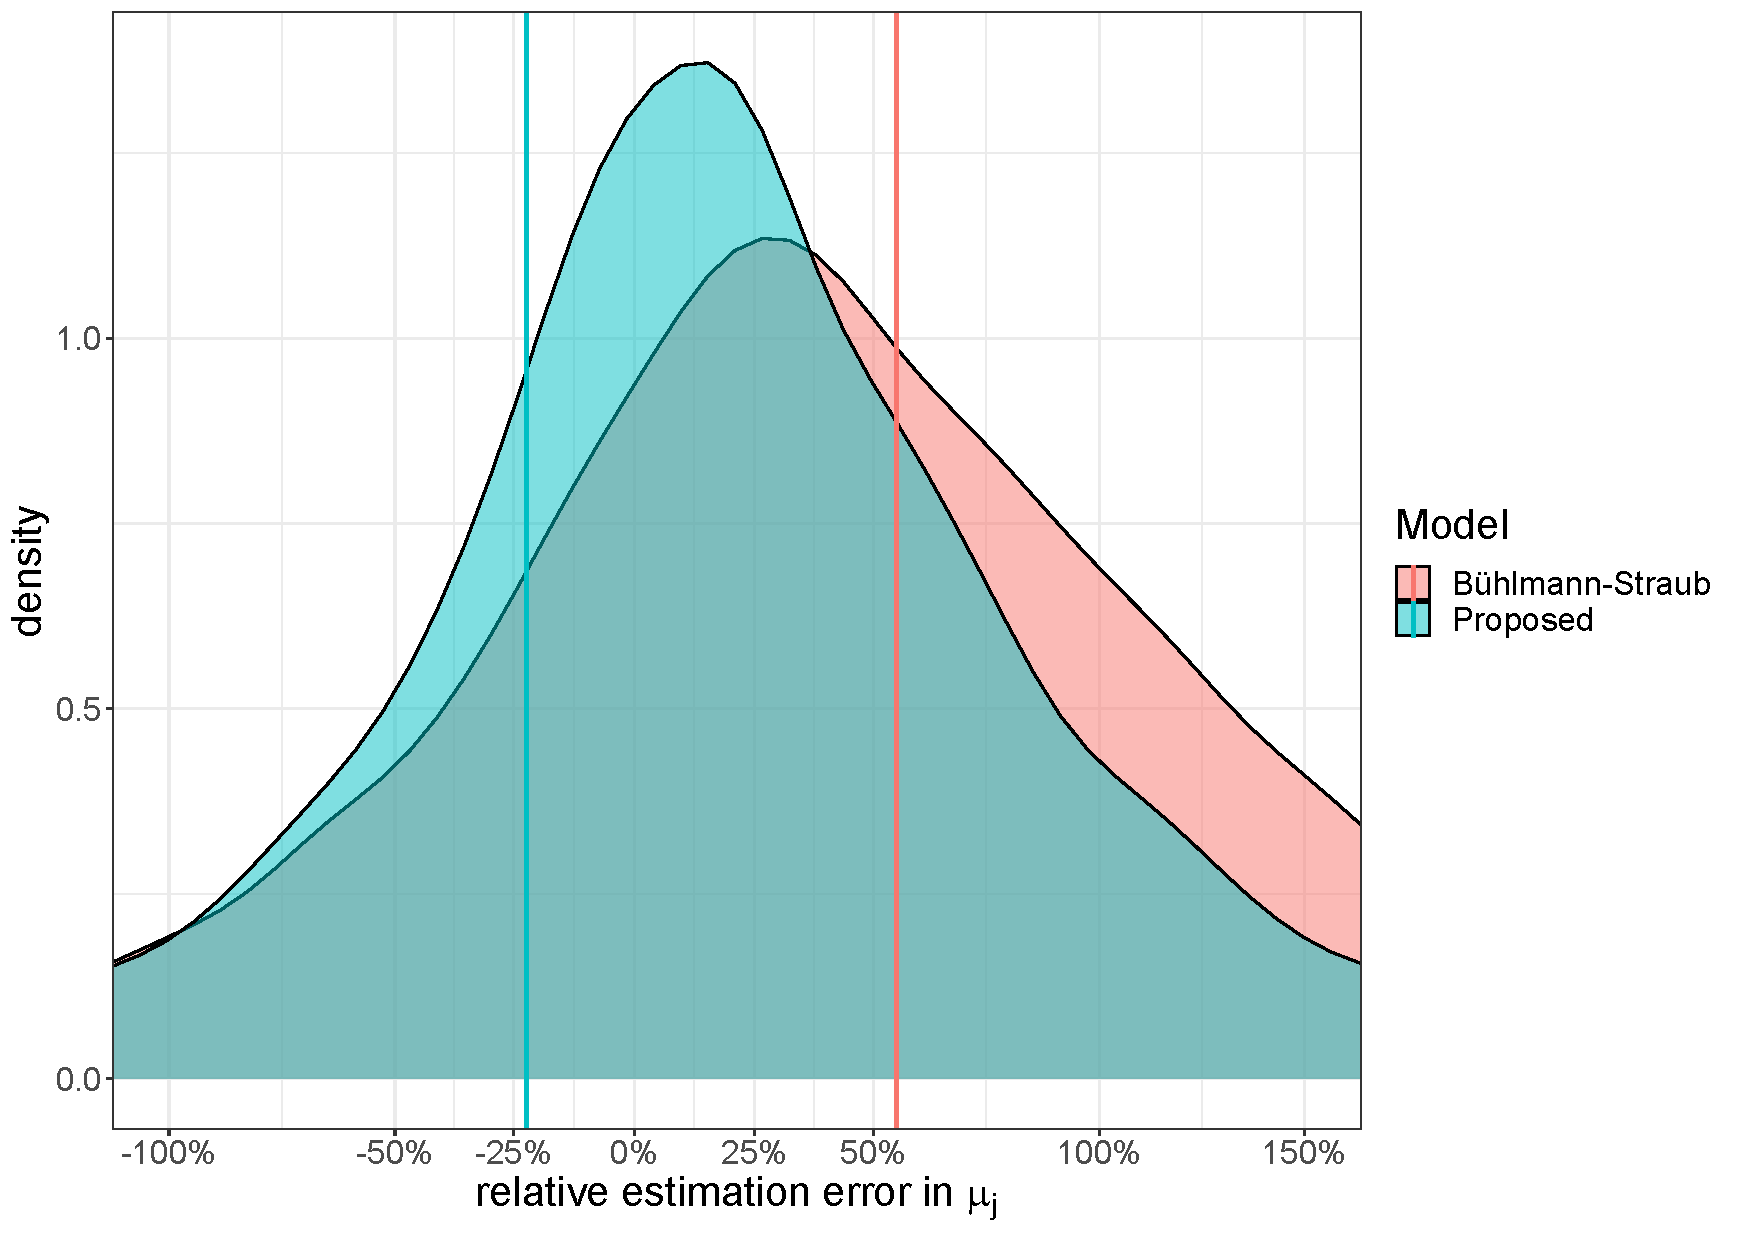
\includegraphics[width=.74\textwidth]{err_dist_muj.pdf}}
  \caption{The distribution of relative error in the estimator $\hat\mu_j^b$ as defined in \eqref{eq:RE_muj} over $10^5$ simulations for the two models. A vertical line is drawn at the average.}
  \label{fig:err_dist_muj}
\end{figure}
\begin{figure}[H]
 \center
 \makebox[\textwidth][c]{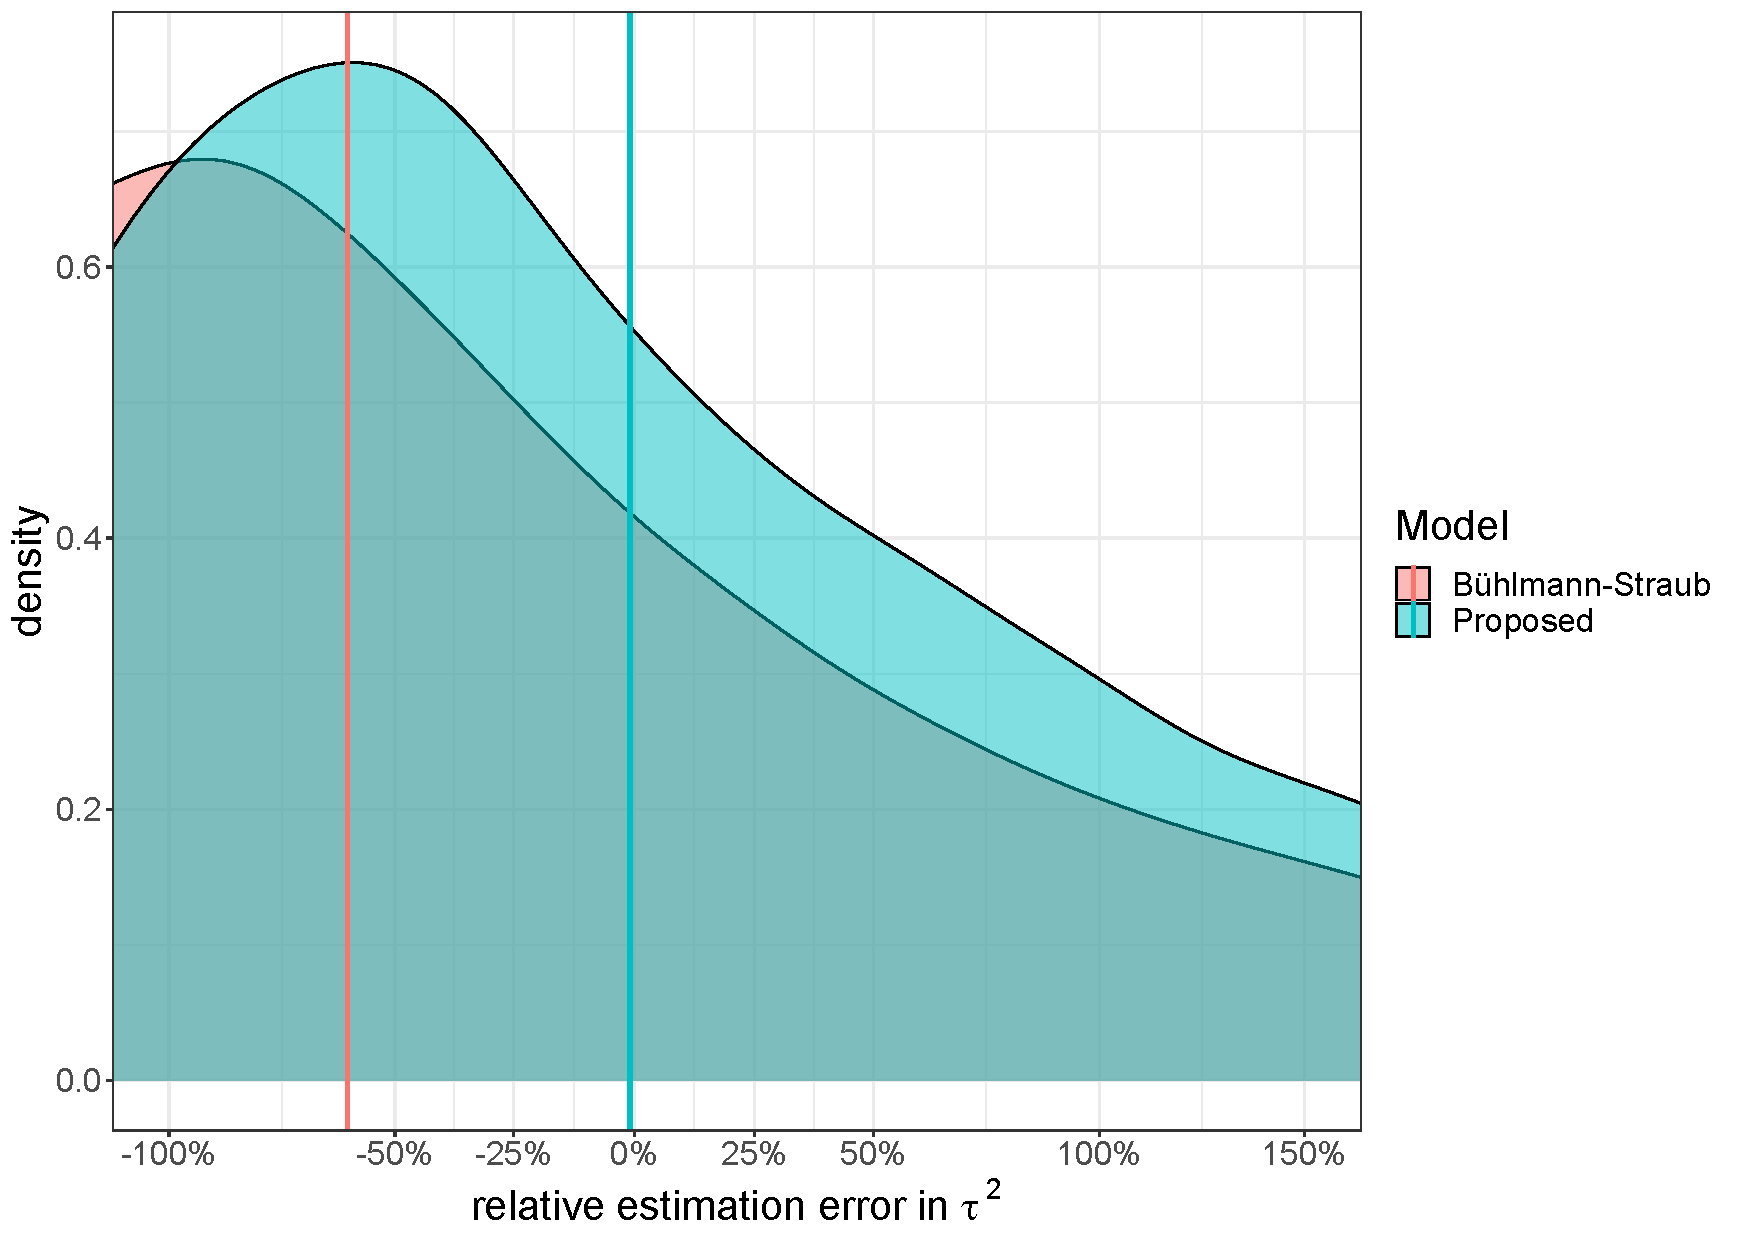
\includegraphics[width=.74\textwidth]{err_dist_tau.pdf}}
  \caption{The distribution of relative error in the estimator $\hat\tau^2$ as defined in \eqref{eq:RE_tau} over $10^5$ simulations for the two models. A vertical line is drawn at the average.}
  \label{fig:err_dist_tau}
\end{figure}
\begin{figure}[H]
 \center
 \makebox[\textwidth][c]{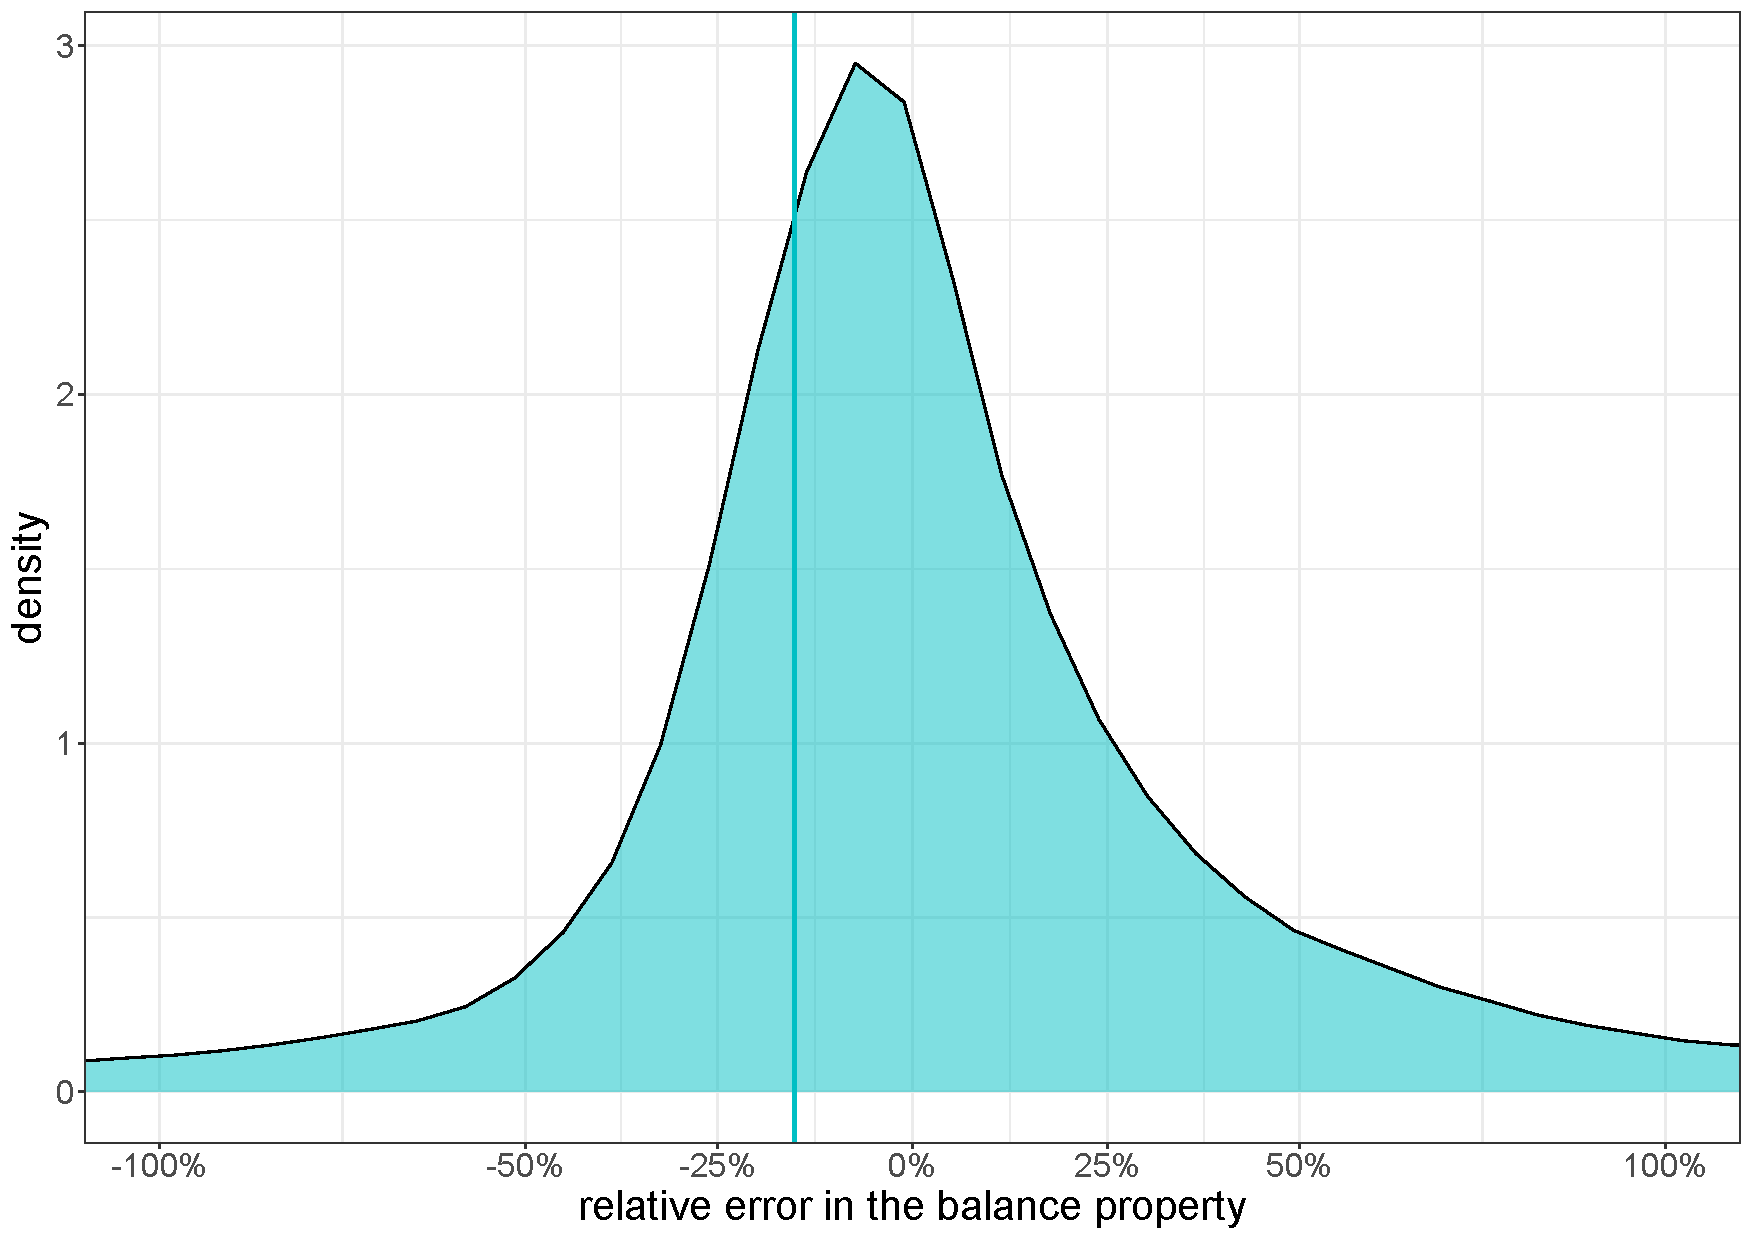
\includegraphics[width=.74\textwidth]{err_dist_bp.pdf}}
    \caption{The distribution of relative error in the balance property as defined in \eqref{eq:RE_bp} over $10^5$ simulations for the proposed model. A vertical line is drawn at the average.}
  \label{fig:err_dist_bp}
\end{figure}

\newpage
\begin{figure}[H]
 \center
 \makebox[\textwidth][c]{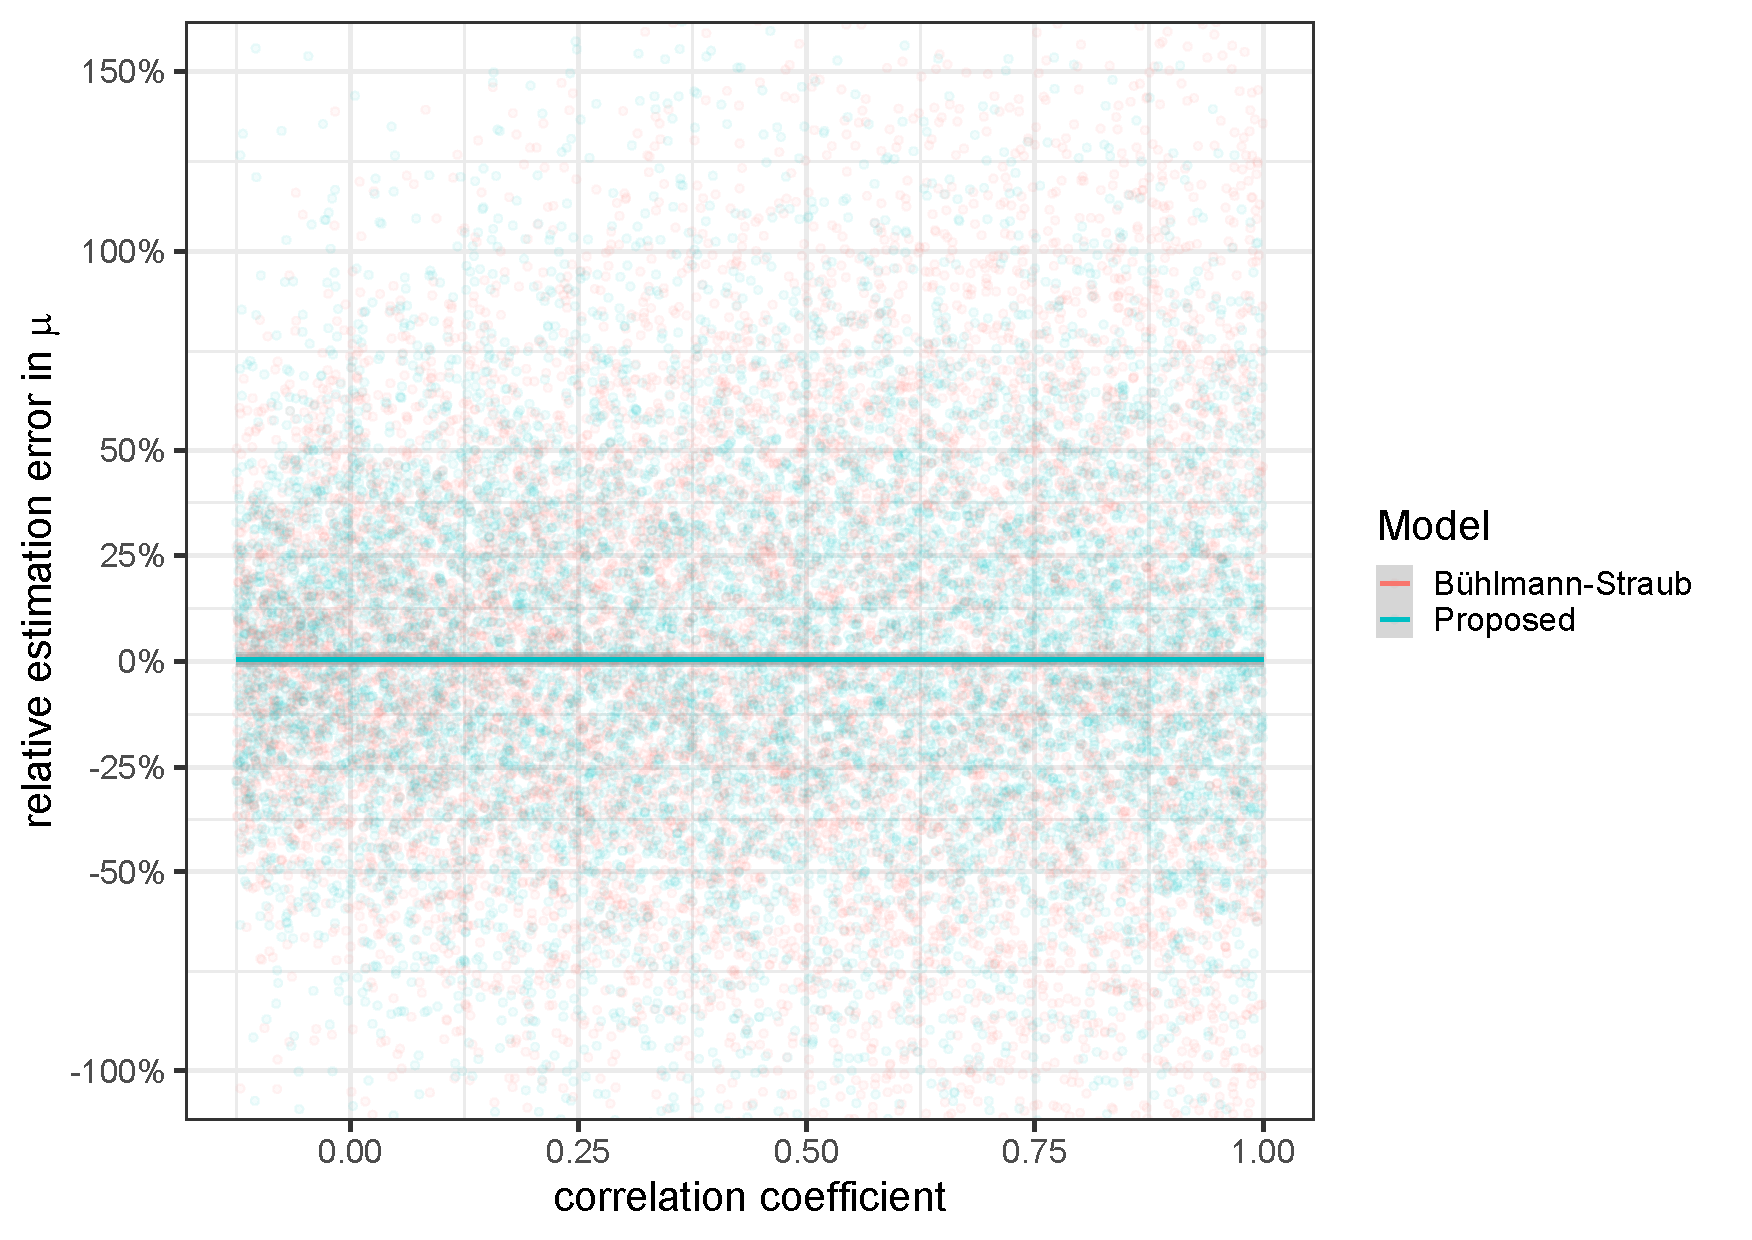
\includegraphics[width=.7\textwidth]{err_trend_mu.pdf}}
  \caption{The $\rho$-dependency of the relative error in the estimator $\hat\mu$ as defined in \eqref{eq:RE_mu} over $10^5$ simulations for the two models. A smooth trend line has been added to help identify local behavior.}
  \label{fig:err_trend_mu}
\end{figure}
\begin{figure}[H]
 \center
 \makebox[\textwidth][c]{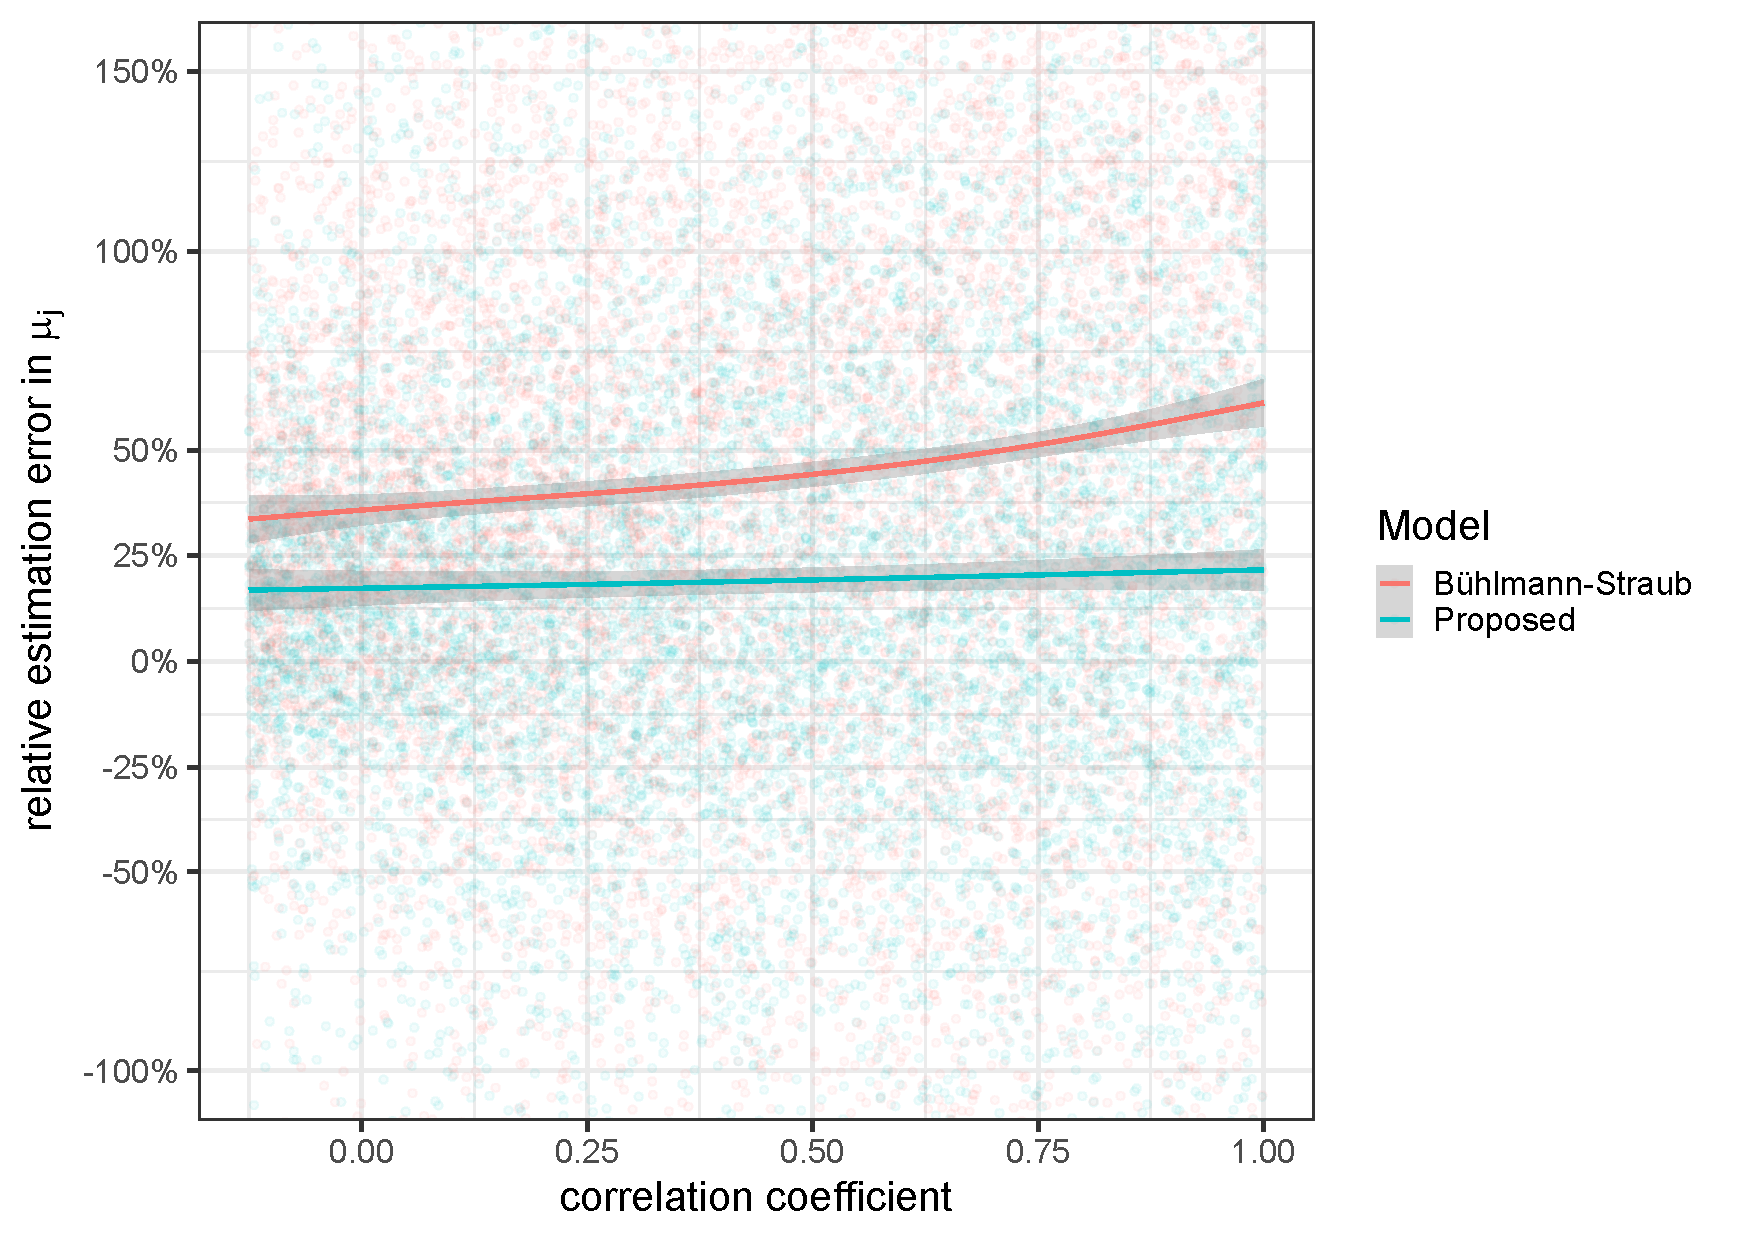
\includegraphics[width=.7\textwidth]{err_trend_muj.pdf}}
 \caption{The $\rho$-dependency of the relative error in the estimator $\hat\mu_j$ as defined in \eqref{eq:RE_muj} over $10^5$ simulations for the two models. A smooth trend line has been added to help identify local behavior.}
  \label{fig:err_trend_muj}
\end{figure}
\begin{figure}[H]
 \center
 \makebox[\textwidth][c]{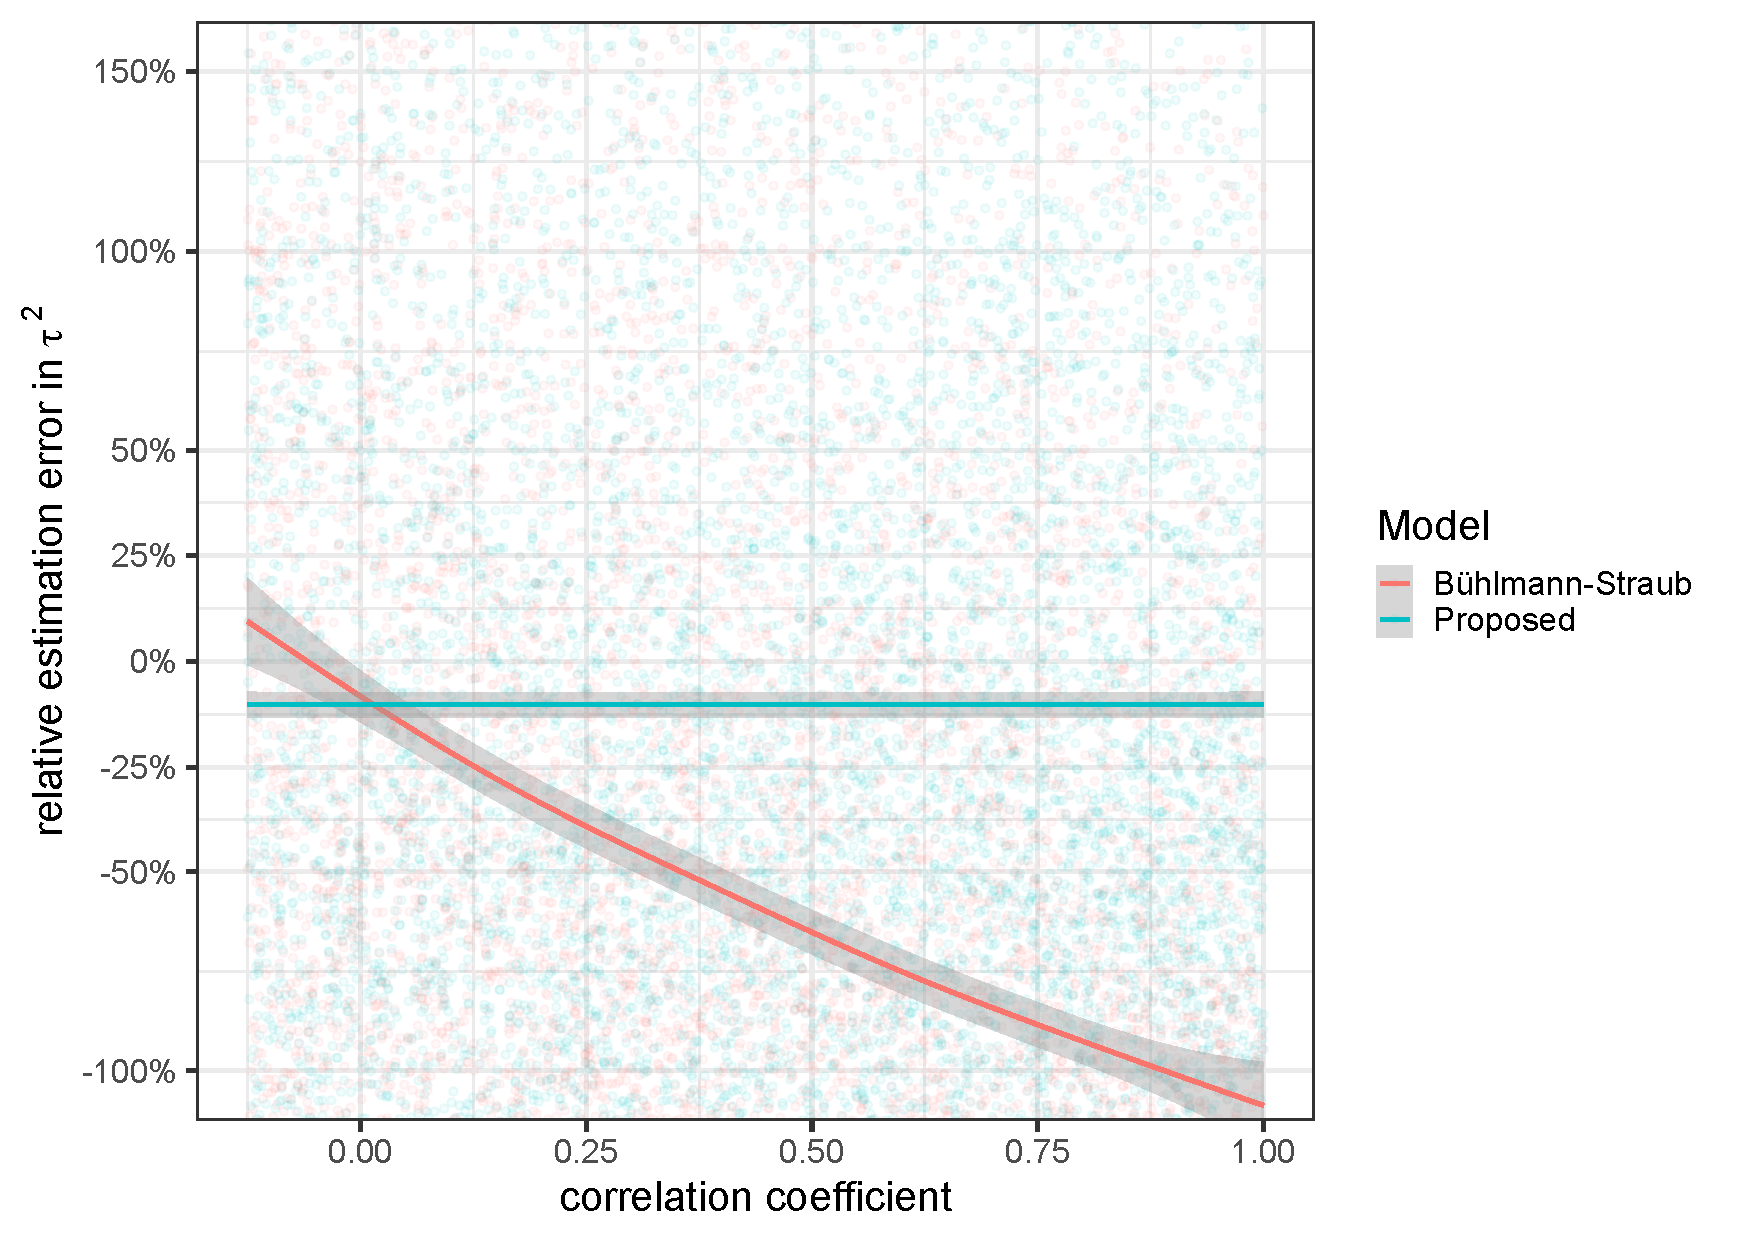
\includegraphics[width=.7\textwidth]{err_trend_tau.pdf}}
 \caption{The $\rho$-dependency of the relative error in the estimator $\hat\tau^2$ as defined in \eqref{eq:RE_tau} over $10^5$ simulations for the two models. A smooth trend line has been added to help identify local behavior.}
  \label{fig:err_trend_tau}
\end{figure}
\begin{figure}[H]
 \center
 \makebox[\textwidth][c]{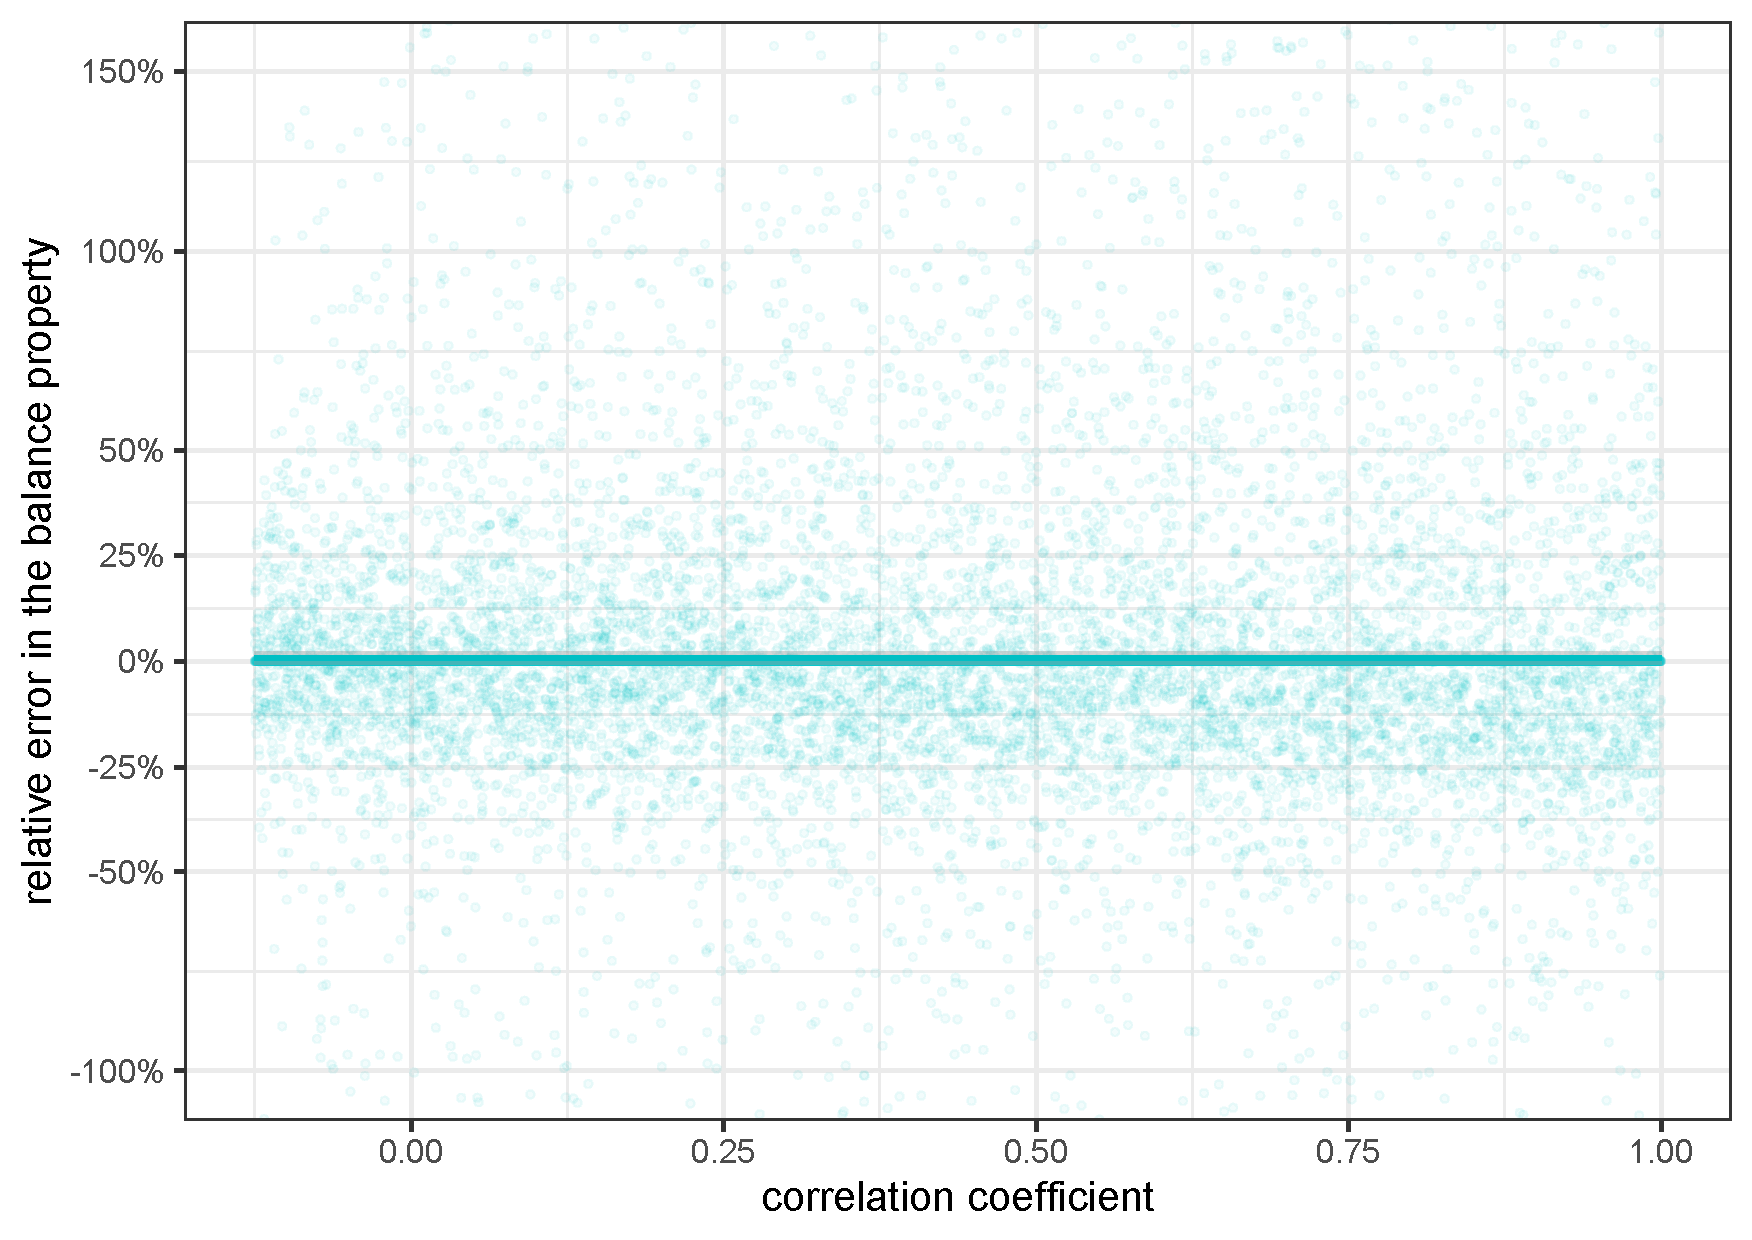
\includegraphics[width=.7\textwidth]{err_trend_bp.pdf}}
  \caption{The $\rho$-dependency of the relative error in the balance property as defined in \eqref{eq:RE_bp} over $10^5$ simulations for the proposed model. A smooth trend line has been added to help identify local behavior.}
  \label{fig:err_trend_bp}
\end{figure}


\newpage
\section{Discussion}
The proposed model extends the homogeneous version of the Bühlmann-Straub model by allowing for correlation between the cohorts and also a more general variance structure. Remember that homogeneous here means that there is a built-in estimator for $\mu$ in the model. The inhomogeneous model takes $\mu$ as known. It was shown that the proposed model is an extension in the sense that the homogeneous Bühlmann-Straub model is included as a special case.

The proposed model is a so-called balanced model. Meaning that the number of terms with data is equal for all cohorts. In other words, $T$ is assumed to be independent of $j$. This assumption was made to simplify the notation and derivation of the estimators.

The basic idea behind the proposed model is to use the correlation between the cohorts to cancel noise and obtain more accurate estimators. This was especially clear in Section \ref{sec:num_ex} where only two cohorts were considered. There we saw that a more extreme correlation could be used to gain superior estimators. It was also shown that when the size of the second cohort was increased the amount of noise that could be canceled when estimating the first cohort was increased. This is different from the classical model where only one credibility coefficient is present in each credibility factor.

It is worth noting that the extension introduced singularities in the credibility factor and weights $\bm b$. For the credibility factor, this happens when the optimal weights $b_j$ imply $\hat\mu_j = \hat\mu$. This point by itself is no problem since any $z_j$ would suffice here. However, it does mean that around this point the credibility factor is unbounded. If $z_j>1$ then the credibility put into $\hat\mu$ is negative. Similarly for $b_j$ since we did not put any bounds on it, it may be optimal to choose $b_j>1$. If this is optimal then it would give $z_j<0$. 

From a practical standpoint, it might seem strange to use negative weights in the calculation of a weighted average. Although from a mathematical standpoint, it is not actually a problem. Consider for instance short-selling in the context of minimum variance portfolios in finance mathematics. When there is a positive correlation, using a negative weight may reduce the variance of the weighted average. This is quite easy to see when looking at the weighting of two variables. It is, of course, possible to apply transformations to $z_j$ and $b_j$, such as ceilings and floors, at the cost of losing accuracy.

The simulation study seems to indicate that the proposed model and the Bühlmann-Straub model are equally well suited for estimating the portfolio average $\mu$. The largest difference between the models is seen when estimating $\mu_j$ using the blended estimator for large overall correlations. It was also noted that the result is quite volatile and ignoring extreme relative errors was needed to more easily compare the models.

It is important to note that the balance property in the homogeneous Bühlmann-Straub model is lost in the general case for the proposed model. The significance of this in practice is however unclear to the author.

The main concern with the proposed model from the author's perspective is the risk of over-parametrization. The bulk of the parameters will be captured by the covariance matrix $ K$ meaning that the number of parameters in the model grows with the square of the number of cohorts. It is not fully understood how much benefit is gained from these added parameters compared to the Bühlmann-Straub model if the data set is limited. A somewhat limited data set was studied in the literature study but further studies are needed to better understand the practical ramifications.

\newpage
\section{Further research}
It is unavoidable at some point to stumble upon a data set with cohort data that spans different ranges. Therefore there should be an alternative formulation of the proposed model that allows for a cohort-dependent time length, i.e.\ the extension $T\rightarrow T_j$. The extension should only have an impact on the estimator of $\sigma_{ij}^2\rho_{ij}$.

Further research is needed to better understand how often unconventional weights (negative or larger than one) occur in practice and how reasonable the final blended estimates are in such cases. It is possible to receive extreme values of the estimators if the parameters are close to a singularity. 

With the above in mind, it could be insightful to look into searching for the optimal weights $\bm b$ under additional constraints. One option is to add the constraint $b_j\geq 0$ for all $j$. Inequality-constrained optimization is unfortunately not as easily solved generally. Alternatives exist, such as optimizing with respect to a transformed variable $\tilde b_j = b_j^2$ which is always non-negative. These modifications would require an adjustment to the credibility factor since $\nu_j=s^2$ would no longer hold. It would also result in a worse expected square error, but it would likely still perform better near the singularities.

Further research is also needed to study the risk of over-parametrization. With this in mind, it would be interesting to study a simplified model with only a single correlation parameter. To pursue this, it is suggested to modify the estimator of the covariance matrix $ K$ accordingly. Some kind of weighted average of the elements $\rho_{ij}$ seems intuitive.


% Add page number in the end of references where needed

% Add abstract and acknowledgements



\newpage
\begin{thebibliography}{99}

\bibitem{esbjorn}
Ohlsson, E., \& Johansson, B. (2010). Non-life insurance pricing with generalized linear models. Berlin: Springer.

\bibitem{buhlmann}
Bühlmann, H., \& Gisler, A. (2005). A course in credibility theory and its applications. Berlin: Springer.

\bibitem{parodi}
Parodi, P., \& Bonche, S. (2010). Uncertainty-based credibility and its applications. Variance.

\bibitem{wen2}
Wen, L., Wu, X., \& Zhou, X. (2009). The credibility premiums for models with dependence induced by common effects. Insurance: Mathematics and Economics.

\bibitem{Oneill}
O'Neill, B. (2021). The Double-Constant Matrix, Centering Matrix and Equicorrelation Matrix: Theory and Applications. arXiv preprint arXiv:2109.05814. Page 18.

\bibitem{wen}
Wen, L., \& Deng, W. (2011). The credibility models with equal correlation risks. Journal of Systems Science and Complexity.

\bibitem{Nurrohmah}
Nurrohmah, S., \& Fithriani, I. (2021). Bühlmann credibility model with correlated risk parameters. In Journal of Physics: Conference Series. IOP Publishing.

\end{thebibliography}


% Weight does not neccesarily need to be the same as the key ratio denominator?

\end{document}  